\documentclass{article}
\usepackage[utf8]{inputenc}
\usepackage[margin=1in]{geometry}
\usepackage[titletoc,title]{appendix}
\usepackage{amsmath,amsfonts,amssymb,mathtools}
\usepackage{graphicx,float}
\usepackage[ruled,vlined]{algorithm2e}
\usepackage{algorithmic}
\usepackage{biblatex}
\usepackage{tikz}
\usepackage{matlab-prettifier}
\usepackage{listings}
\usepackage{xcolor}
\usepackage{hyperref}
\usepackage{caption}
\usepackage{subfig}
\addbibresource{references.bib}

\newcommand{\hmwkTitle}{Homework 4}
\newcommand{\hmwkDueDate}{March 16, 2020}
\newcommand{\hmwkClass}{Computational Methods for Data Analysis}
\newcommand{\hmwkClassNum}{AMATH 582}
\newcommand{\hmwkClassInstructor}{Professor J. Nathan Kutz}
\newcommand{\hmwkAuthorName}{\textbf{Chandan Sharma Subedi}}
\newcommand{\hmwkClassSection}{Section A}

%
% Title Page
%

\title{
    \vspace{2in}
    \textmd{\textbf{\hmwkClass}}\\
    \vspace{0.3in}\textmd{\textbf{\hmwkTitle}}\\
    \normalsize\vspace{0.1in}\small{Due\ on\ \hmwkDueDate\ at 5:00pm}\\
    \vspace{0.1in}\large{\textit{\hmwkClassInstructor}} \\
    \vspace{0.1in}\large{{\hmwkClassSection}} \\
    \vspace{2.5in}
}

\author{\hmwkAuthorName}
\date{}

\begin{document}

\maketitle
\pagebreak

% Abstract
\begin{abstract}
In this paper Singular Value Decomposition (SVD) was analyzed as an unsupervised learning algorithm in the context of facial recognition and music genre classification. A Naive Bayes classification algorithm was implemented to classify the genre of a $5$ sec sample of music.

\end{abstract}

% Introduction and Overview
\section{Introduction and Overview}
Singular Value Decomposition (SVD) is one of the most widely used unsupervised learning algorithm. It is also heavily used in optimization, signal analysis and numerical computation. This paper explores the fundamental idea behind SVD through its application as a learning algorithm. The first part of the paper discusses how SVD can be used for facial recognition. In this problem, SVD is applied to a large set of images to extract out dominant modes. The decomposition gives rise to a new coordinate system, also know as the set of eigenfaces. These eigenfaces are extremely effective for facial recognition.

The second part of the paper delves into the area of music genre classification. It is extremely easy for us to identify the genre of the music aftet we hear it. However, it is not clear as to how our mind processes all the information instantly. The objective is to implement and train a Naive Bayes classifier that can classify a $5$ sec sample of music. The scope of the problem is limited to $3$ genres of music: Classical Rock, Jazz and Grunge.


%  Theoretical Background
\section{Theoretical Background}\label{Theory}
Singular Value Decomposition is a matrix decomposition of the form
\begin{align*}
\begin{bmatrix}
&&\\
&&\\
&\textbf{A}& \\
&&\\
&&\\
\end{bmatrix}
\begin{bmatrix}
&&\\
&&\\
&\mathbf{v_1}& \mathbf{v_2}& \hdots & \mathbf{v_n}&\\
&&\\
&&\\
\end{bmatrix}
&=
\begin{bmatrix}
&&\\
&&\\
&\mathbf{u_1}& \mathbf{u_2}& \hdots & \mathbf{u_n}&\\
&&\\
&&\\
\end{bmatrix}
\begin{bmatrix} 
\mathbf{\sigma_1}&&\\
&\mathbf{\sigma_2}&\\
&& \ddots \\
&&&& \\
&&&&\mathbf{\sigma_n}\\
\end{bmatrix} \\
\mathbf{AV} &= \mathbf{U\Sigma} \\
\mathbf{A} &= \mathbf{U\Sigma V^{*}}
\end{align*}
The matrix $\mathbf{\Sigma}$ is an $m$ x $n$ diagonal matrix with positive entries provided the matrix \textbf{A} is of full rank. It stores the singular values, representing the stretching space, ordered from largest to smallest so that $\sigma_1 \ge \sigma_2 \ge ... \ge \sigma_n$. The matrix \textbf{U} is a $m$ x $n$ unitary matrix with orthonormal columns (left-singular vectors). The matrix \textbf{V} is an $n$ x $n$ unitary matrix with orthonormal columns (right-singular vectors). Both of these vectors represent rotation. Furthermore, $\mathbf{v_1}$ is the vector that, when multiplied with the matrix A, strectches by a factor of $\mathbf{\sigma_1}$ and rotates so that it points along $\mathbf{u_1}$. Therefore columns of matrix \textbf{V} are the principal components of the matrix \textbf{A}. \\

The discrete Gabor Tranform discretizes the signal through sliding window. Each window captures a piece of the signal, which is then fourier tranformed to gives its frequency spectrum. As we slide the window through the signal, we obtain a varying frequency spectrum. Combining these spectrums, we obtain a spectrogram that gives us a visual representation of how frequency spectrum varies over time in the signal.

The Gabor Transform of the function $f(t)$ is defined as
\begin{align*}
&G_f(\tau, k) = \int_{-\infty}^{\infty} f(t)\overline{g}_a(\tau - t)e^{-ikt} dt 
\end{align*}
$g_a(\tau - t)$ is the sliding window obtained through the parameterization of function $g(t)$ over a scaling factor $a$ and a shifting factor $\tau$. The scaling factor $a$ determines the width of the window. In this assingment, the gaussian sliding window ($g_a(\tau - t) = e^{-a(\tau - t)^2}$) was used.

When we mulitply the signal with these functions, the signal that lies inside the window remains more or less unchanged, while the signal that lies outside the window approaches zero. Thus, these functions act as a window that isolates a part of a signal at a particular instance of time.

A spectrogram is generated by combining frequency spectrums obtained through the fourier tranform of windowed signals. Thus, it gives a visual representation of how frequency spectrum is changing over time. The resolution of spectrogram, obtained through Gabor Transform, depends strongly on the sliding window and its scaling and sliding parameters. This stems from the fact that the fundamental idea of Gabor Transform is to make some compromise on spectral resolution so as to gain some temporal resolution. \\

Naive Bayes algorithm is a supervised classification algorithm based on Bayes theorem that assumes independence among features. The algorithm is most often used in the text classification and recommender systems. While the assumption of independence among features is highly undesirable, the algorithm benefits from its easy implementation and scalability.


% Algorithm Implementation and Development
\section{Algorithm Implementation and Development}\label{Algorithm}
\subsection{Eigenfaces}
In order to study eigenfaces, Yale Faces B database was used. The database consisted of large sets of cropped and un-cropped grayscale images. The analysis was implemented through following steps:
\begin{itemize}
\item Each image was reshaped into a large column vector. The image was normalized by subtracting its mean from each element.
\item The mean-subtracted image vectors were horizontally stacked to create the matrix $X$.
\item SVD (economic) was performed on the matrix. Energy content of each mode and r-rank approximations were plotted.
\end{itemize}


\subsection{Music Genre Classification}
A music database was created, containing music clips from three different genre of music: Classic Rock, Grunge and Jazz. A naive bayes classifier was implemented to classify the music genre under 3 different training conditions:
\begin{itemize}
\item Test 1: Train NB classifier with music from three bands of different genres.
\item Test 2: Train NB classifier with music from three bands of the same genre.
\item Test 3: Train NB classifier with music from multiple bands of different genres.
\end{itemize}

The implementation involved three key steps: \\

\textbf{Generate spectrogram of all music:} \\
All music clips were loaded and re-sampled to reduce computation time. A Gabor filter, based on Gaussian sliding window, was implemented to generate the spectrogram of the clip. All spectrograms were stacked in a matrix for SVD decomposition. \\

\textbf{Find principal components:} \\
An economy-size SVD decomposition was computed using MATLAB built in function \emph{svd}. Energy contents of each mode were plotted to identify the number of modes $n$ needed for classification. \\

\textbf{Implement Naive Bayes classifier:}\\
The music data was randomly split into testing and training datasets. A NB classifier object was created and trained using MATLAB in-built function \emph{fitcnb}. The classifier object was used to predict the classification of test data. Error was estimated through cross-validation. Error distribution was computed by repeating the classification (with random data splitting) 100 times.


% Computational Results
\section{Computational Results}\label{Result}
\subsection{Eigenfaces}
All the images, except one folder that was later used for test images, were transformed into the matrix as explain above. 
Figure \ref{fig:eigfac1} shows first 5 eigenfaces of cropped and un-cropped images respectively. Eigenfaces are the columns of the left-singular matrix \textbf{U}. They define a new co-ordinate system. The diagonal matrix $\mathbf{\Sigma}$ contains singular values that represent the energy content of these eigenfaces, while \textbf{V} represent principal components of the matrix $X$. \\

\begin{figure}[!t]
\centering
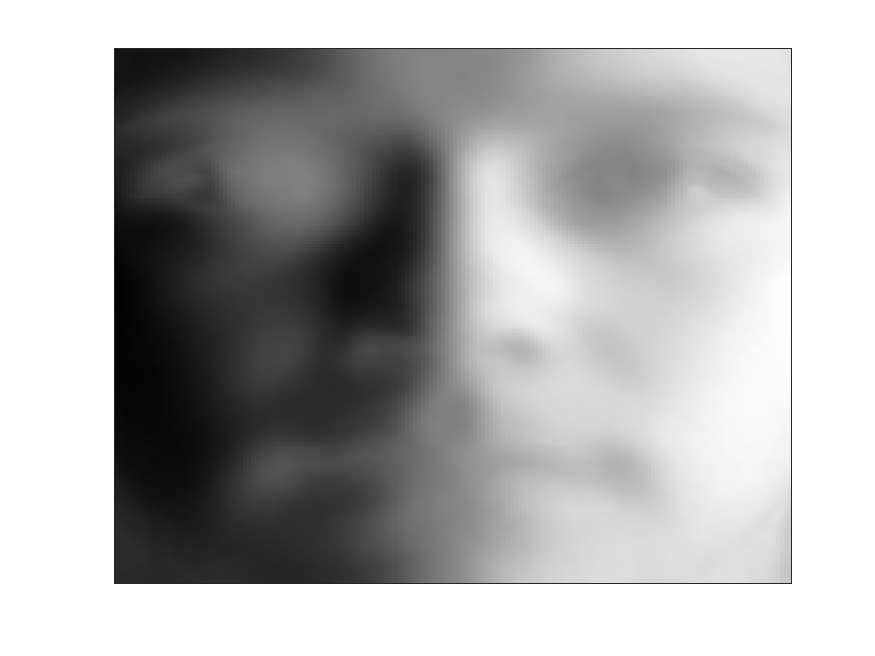
\includegraphics[width = 0.18\linewidth]{./Figures/cropped1.png}
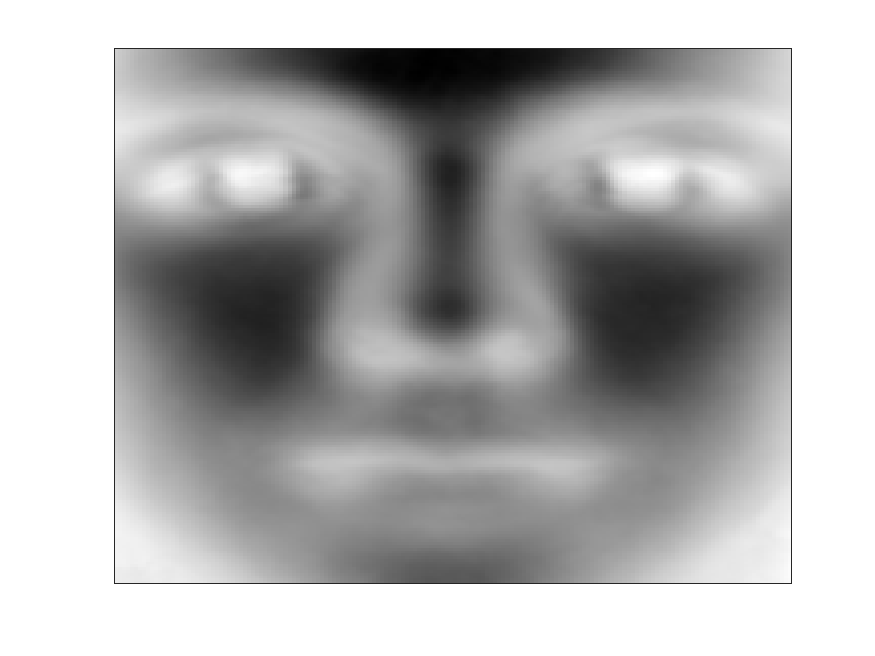
\includegraphics[width = 0.18\linewidth]{./Figures/cropped2.png}
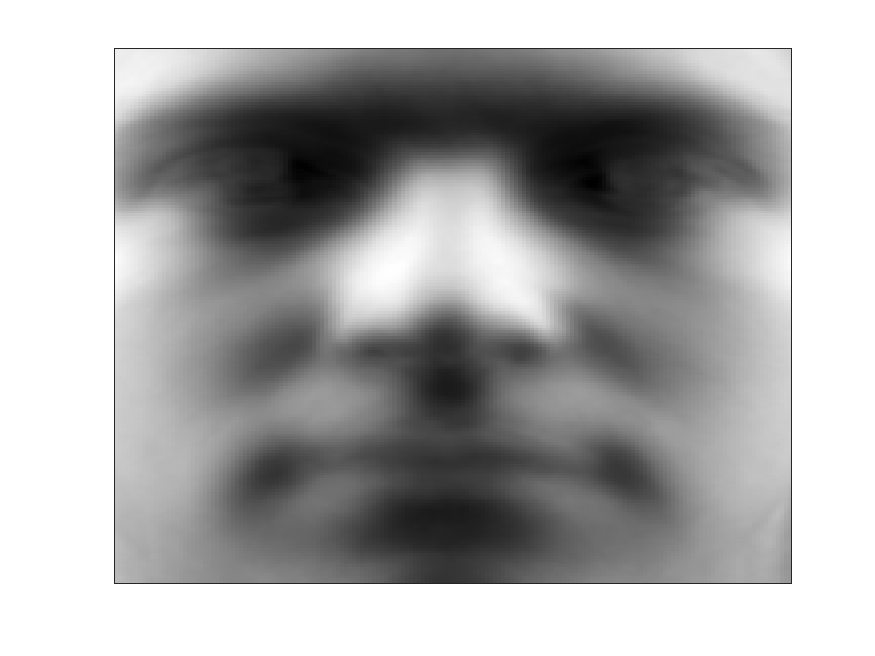
\includegraphics[width = 0.18\linewidth]{./Figures/cropped3.png}
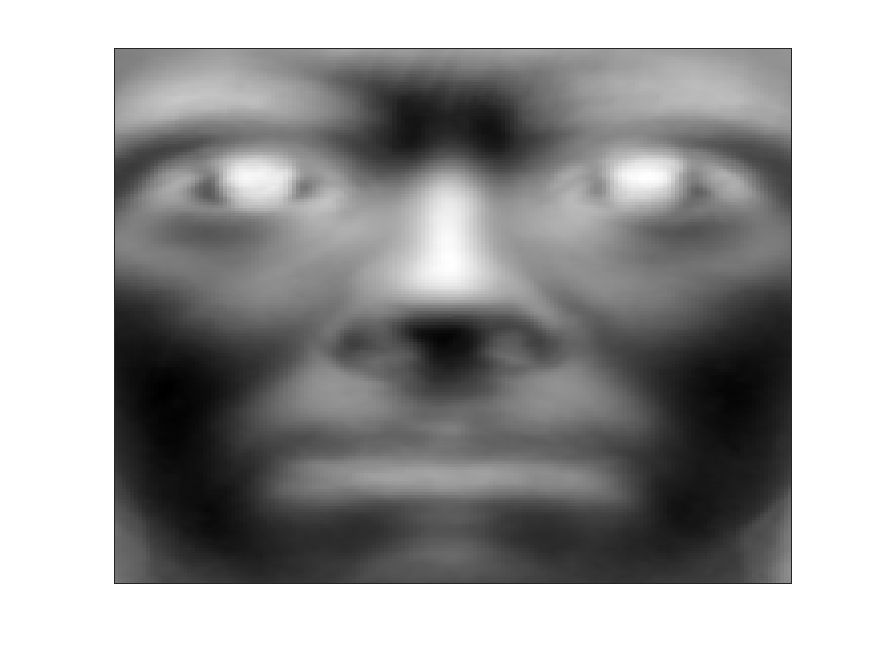
\includegraphics[width = 0.18\linewidth]{./Figures/cropped4.png}
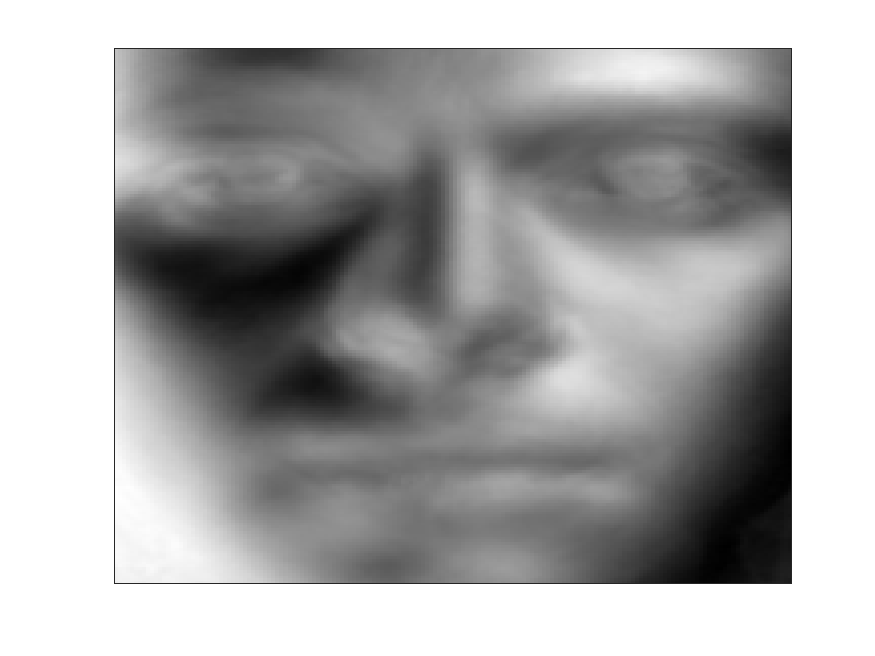
\includegraphics[width = 0.18\linewidth]{./Figures/cropped5.png}
\caption{First 5 eigenfaces of the matrix $X$ for cropped images dataset.}
\label{fig:eigfac1}
\end{figure}

A test image that was not in the training set was projected onto the eigenface subspace. Figure \ref{fig:rapprox} shows r-rank approximations of the test image, i.e projection of test image onto the firsts r-PCA modes. It was found that for cropped image dataset, 128 modes were necessary to capture 50 \% of the total energy. Similar analysis of un-cropped images produced eigenfaces as shown in the figure \ref{fig:eigfac2}. However, they are drastically different. Due to misalignment, reflection and large background in images, SVD was forced to extract those non-facial feactures as well. Furthermore, it was found that for un-cropped image dataset, 19 modes were necessary to capture 50 \% of the total energy. Those dominant modes may not represent facial features but instead, may represent (as an example) a round object in the image.
\begin{figure}[!t]
\centering
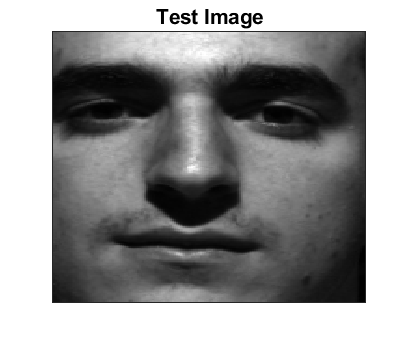
\includegraphics[width = 0.18\linewidth]{./Figures/test1.png}
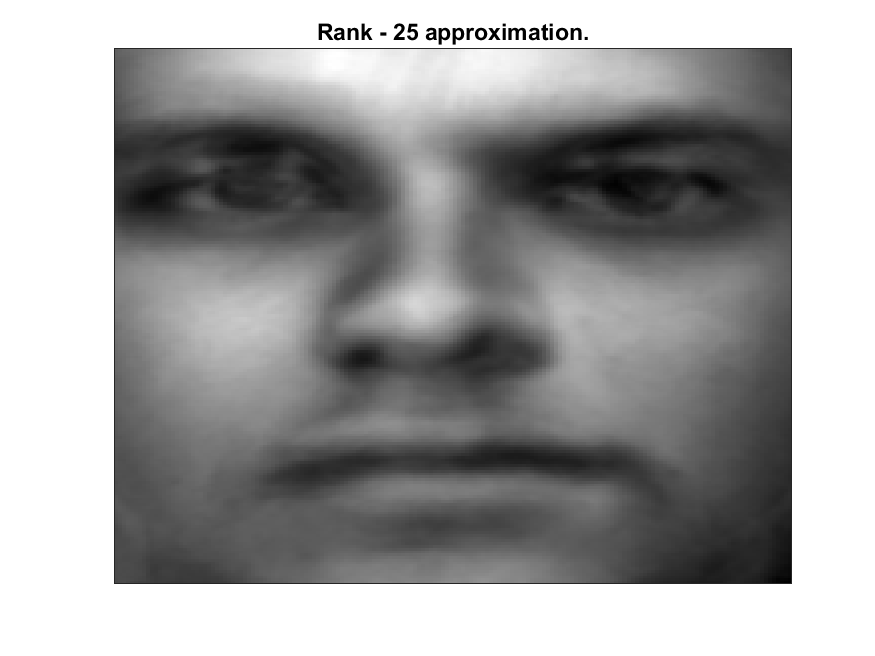
\includegraphics[width = 0.18\linewidth]{./Figures/r25.png}
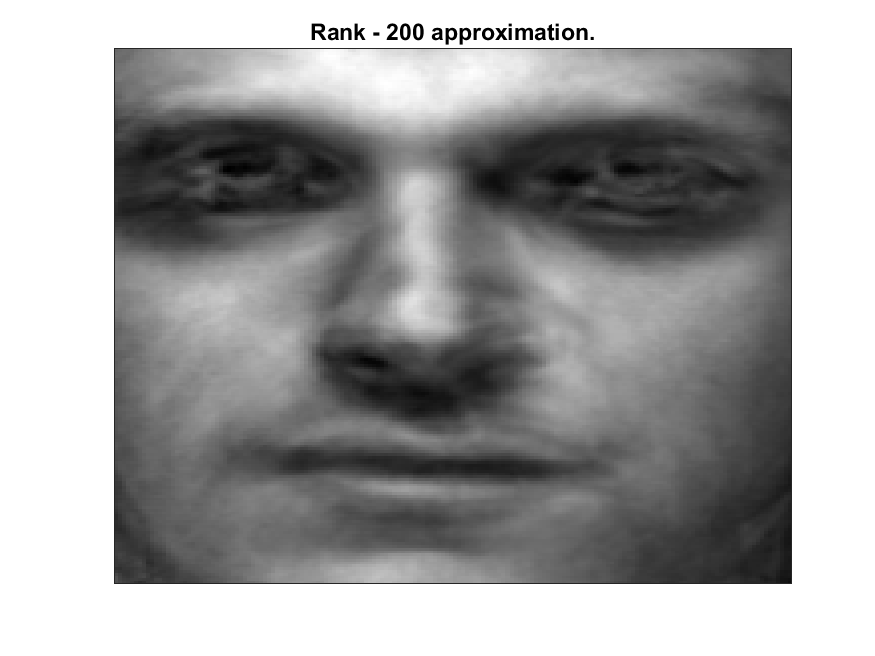
\includegraphics[width = 0.18\linewidth]{./Figures/r200.png}
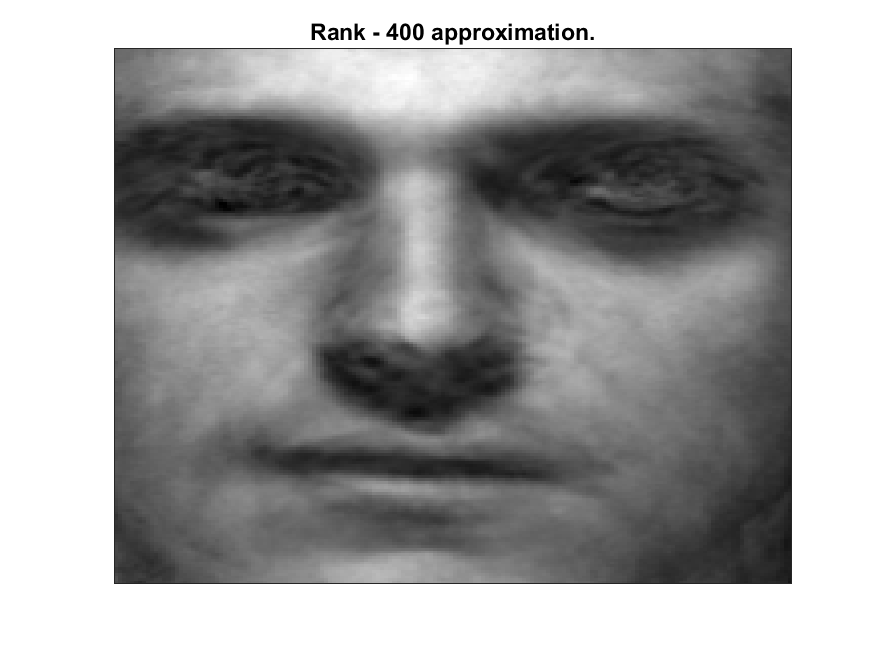
\includegraphics[width = 0.18\linewidth]{./Figures/r400.png}
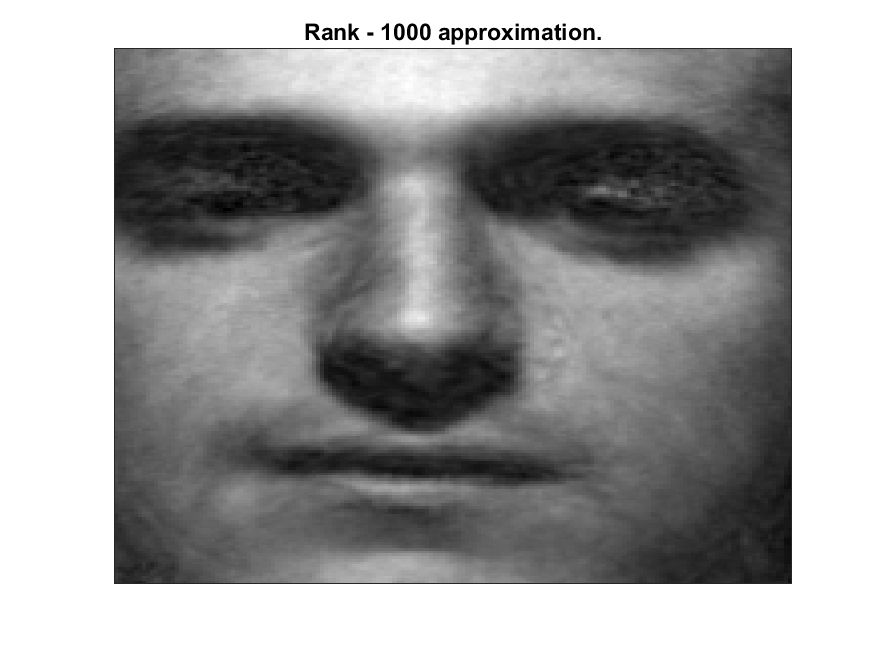
\includegraphics[width = 0.18\linewidth]{./Figures/r1000.png}
\caption{Rank-r approximations of the test image.}
\label{fig:rapprox}
\end{figure}


\begin{figure}[!t]
\centering
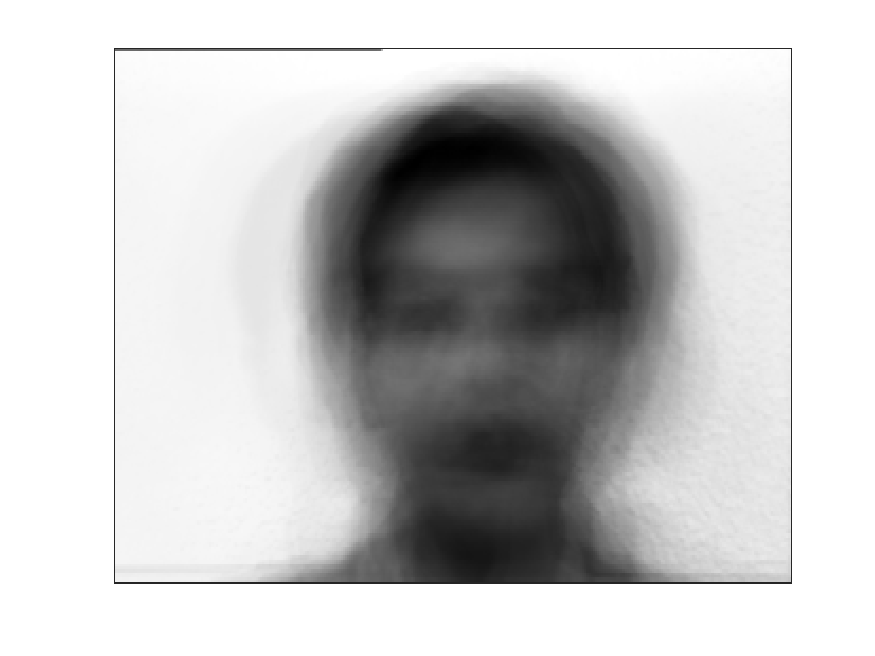
\includegraphics[width = 0.18\linewidth]{./Figures/uncropped1.png}
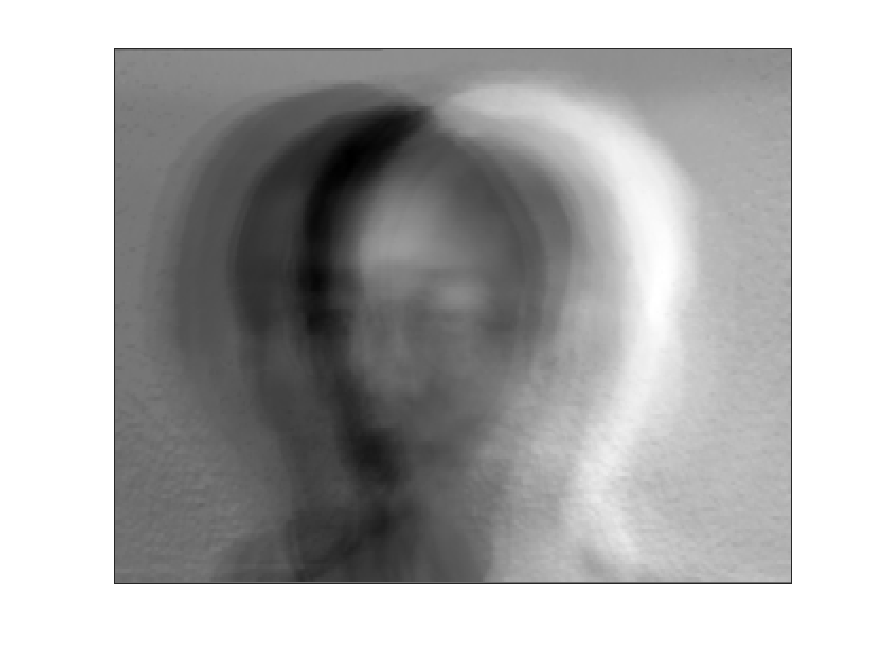
\includegraphics[width = 0.18\linewidth]{./Figures/uncropped2.png}
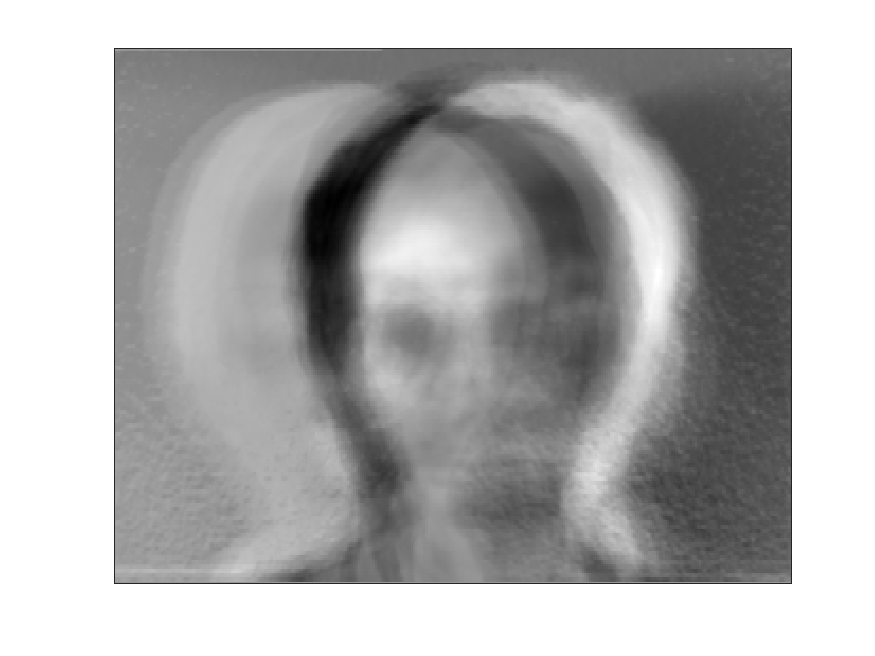
\includegraphics[width = 0.18\linewidth]{./Figures/uncropped3.png}
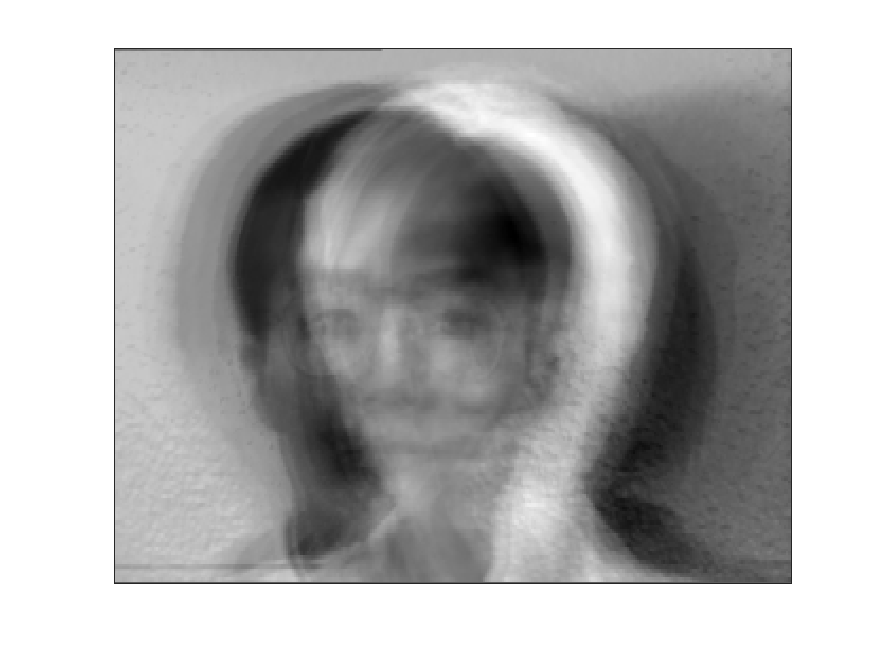
\includegraphics[width = 0.18\linewidth]{./Figures/uncropped4.png}
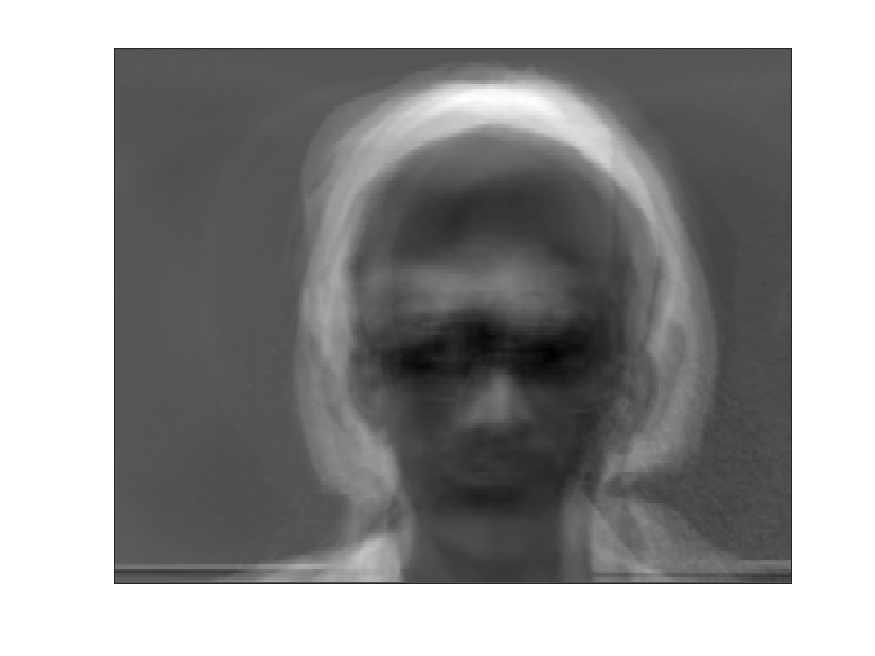
\includegraphics[width = 0.18\linewidth]{./Figures/uncropped5.png}
\caption{First 5 eigenfaces of the matrix $X$ for un-cropped images dataset.}
\label{fig:eigfac2}
\end{figure}

\subsection{Music Genre Classification}
All the music clips were downsampled by a factor of $2$ to maintain a resonable computation time. The Gaussian sliding window, used for the Gabor Transform, was parameterized by the window width of $a = 100$ and sliding time-step $\tau = 0.1$. Figure \ref{fig:Nirvana} shows the spectrogram of all Nirvana music clips. \\

\begin{figure}[!t]
\centering
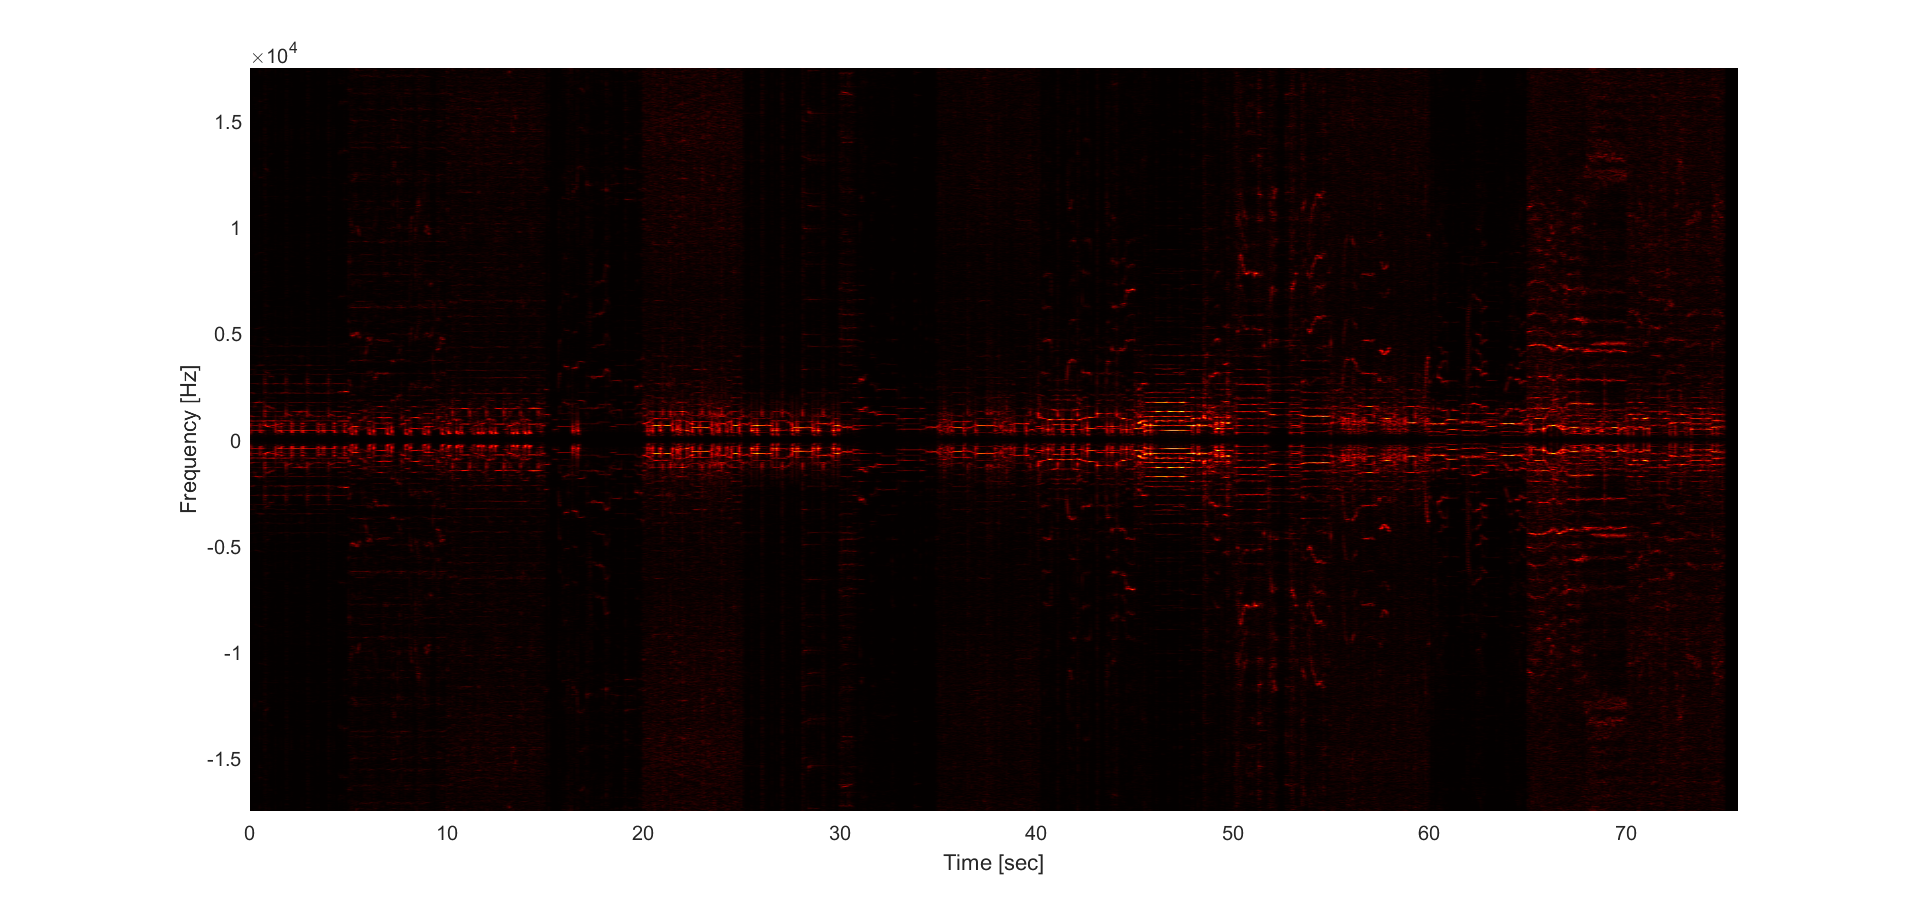
\includegraphics[width = \linewidth]{./Figures/spectrogram.png}
\caption{Spectrogram of all Nirvana music clips.}
\label{fig:Nirvana}
\end{figure}

\pagebreak
\textbf{Test 1: Train NB classifier with music from three bands of different genres.}
Figure \ref{fig:test1}(a) shows the percentage of total energy contained in each modes. It was found that the classification error was smallest when $7$ principal components were used. The accurancy of NB classifier was found to be $\approx 65 \%$ with standard deviation of $\approx 10 \%$. Figure \ref{fig:test1}(b) shows how much the first $3$ principal components of the music of three bands from different genre are correlated. While one cluster seems to be distinct, the other two clusters were much overlap. \\

\begin{figure}[!b]
\subfloat[Percentage of variance captured by each mode.]{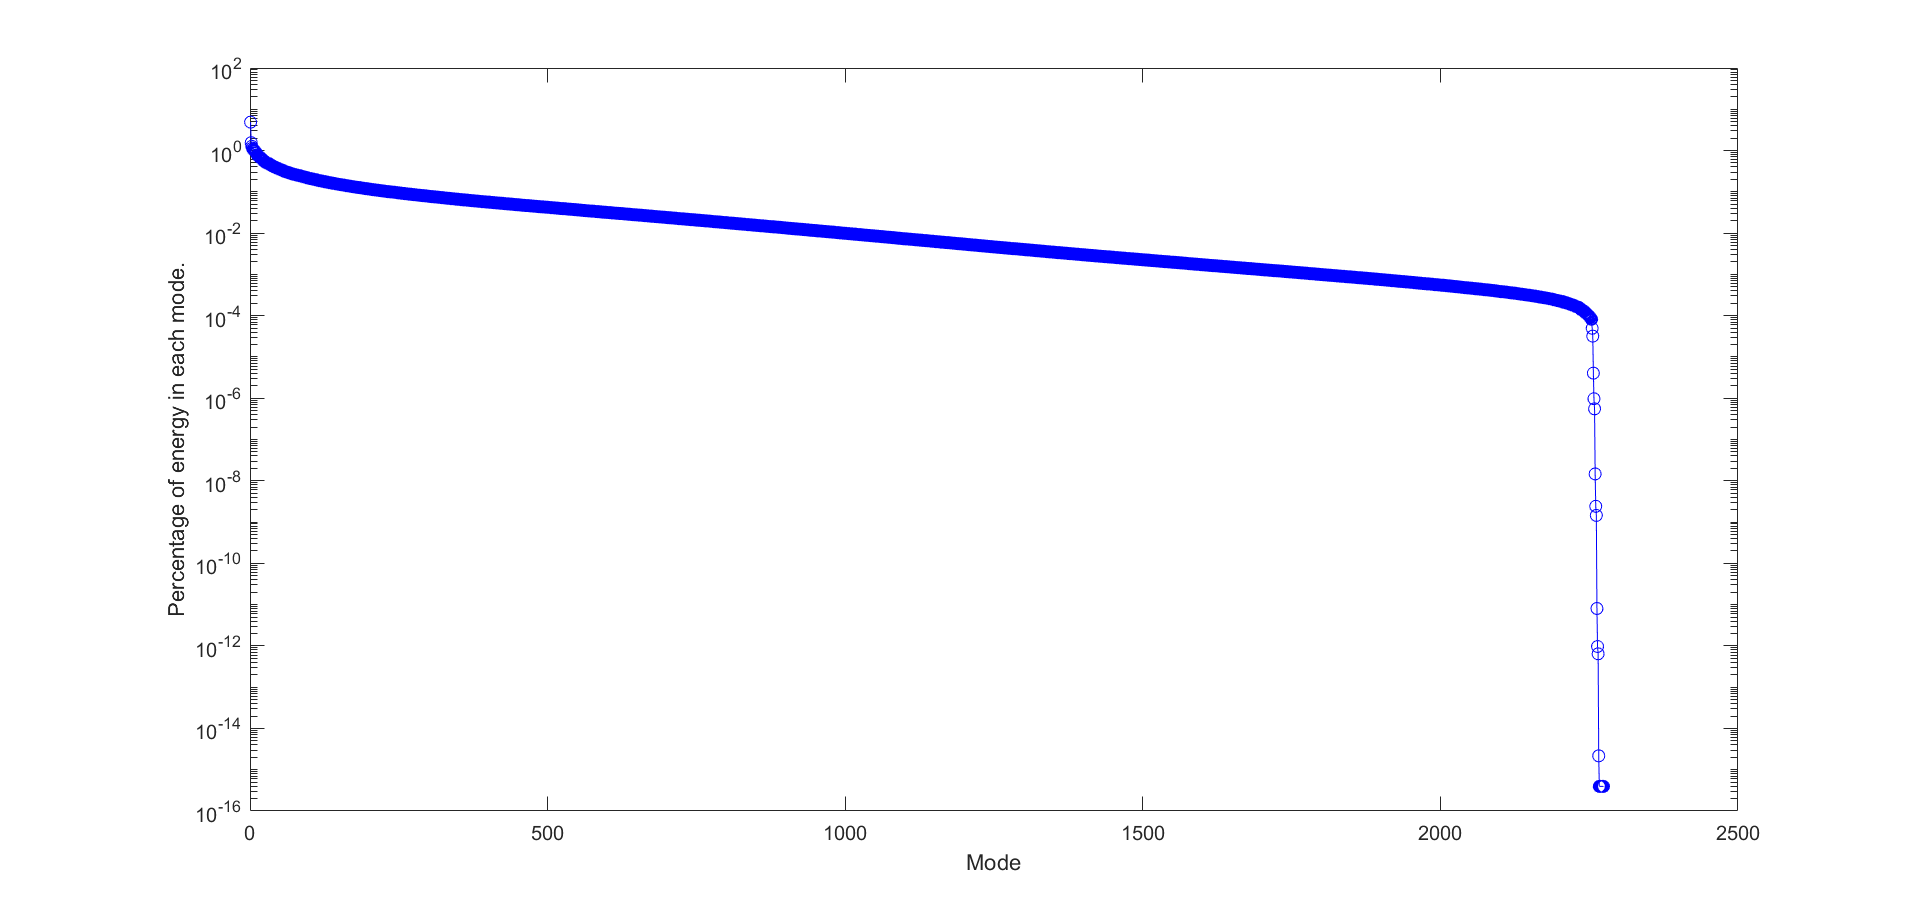
\includegraphics[width = 0.5\linewidth]{./Figures/test1_sigma.png}} 
\subfloat[First 3 principal components.]{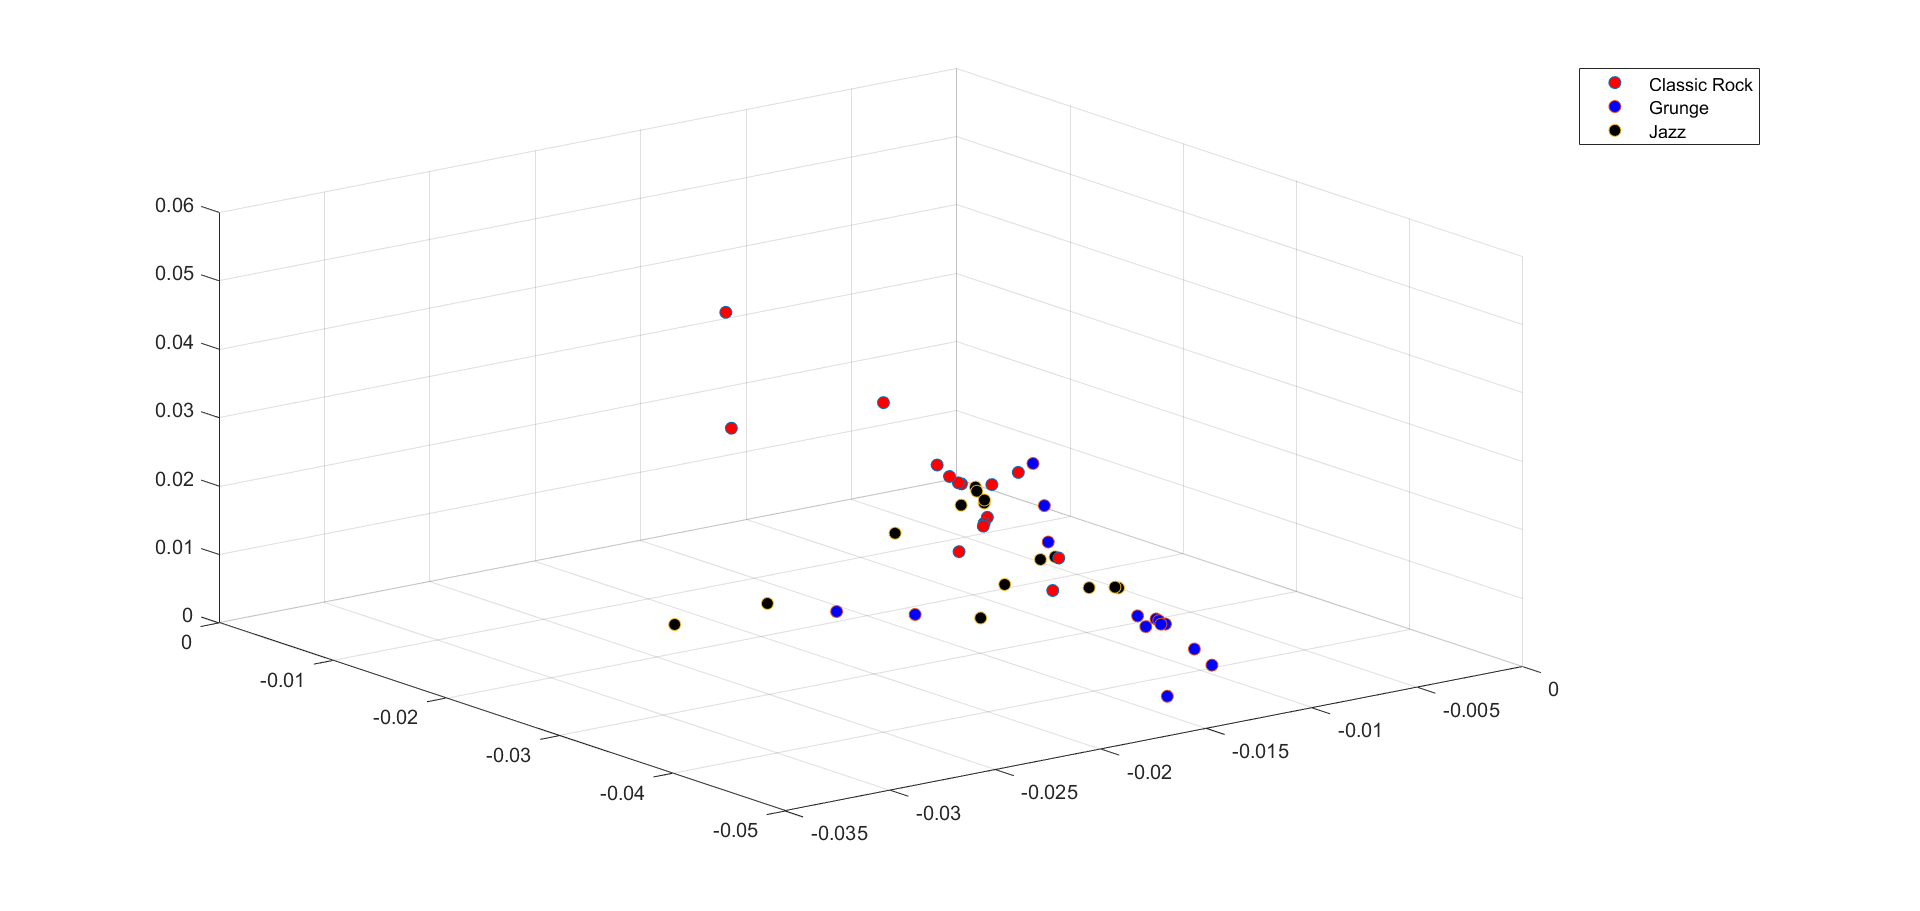
\includegraphics[width = 0.5\linewidth]{./Figures/test1_modes.png}}
\caption{Principal Component Analysis for Test 1. NB clasifier was trained with music from three bands of different genre.}
\label{fig:test1}
\end{figure}


\textbf{Test 2: Train NB classifier with music from three bands of same genre.}
Figure \ref{fig:test2}(a) shows the percentage of total energy contained in each modes. It was found that the classification error was smallest when $7$ principal components were used. The accurancy of NB classifier was found to be $\approx 59 \%$ with standard deviation of $\approx 14 \%$. Figure \ref{fig:test2}(b) shows how much the first $3$ principal components of the music of three bands from different genre are correlated. The clusters are very much overlapped. \\

\begin{figure}[!t]
\subfloat[Percentage of variance captured by each mode.]{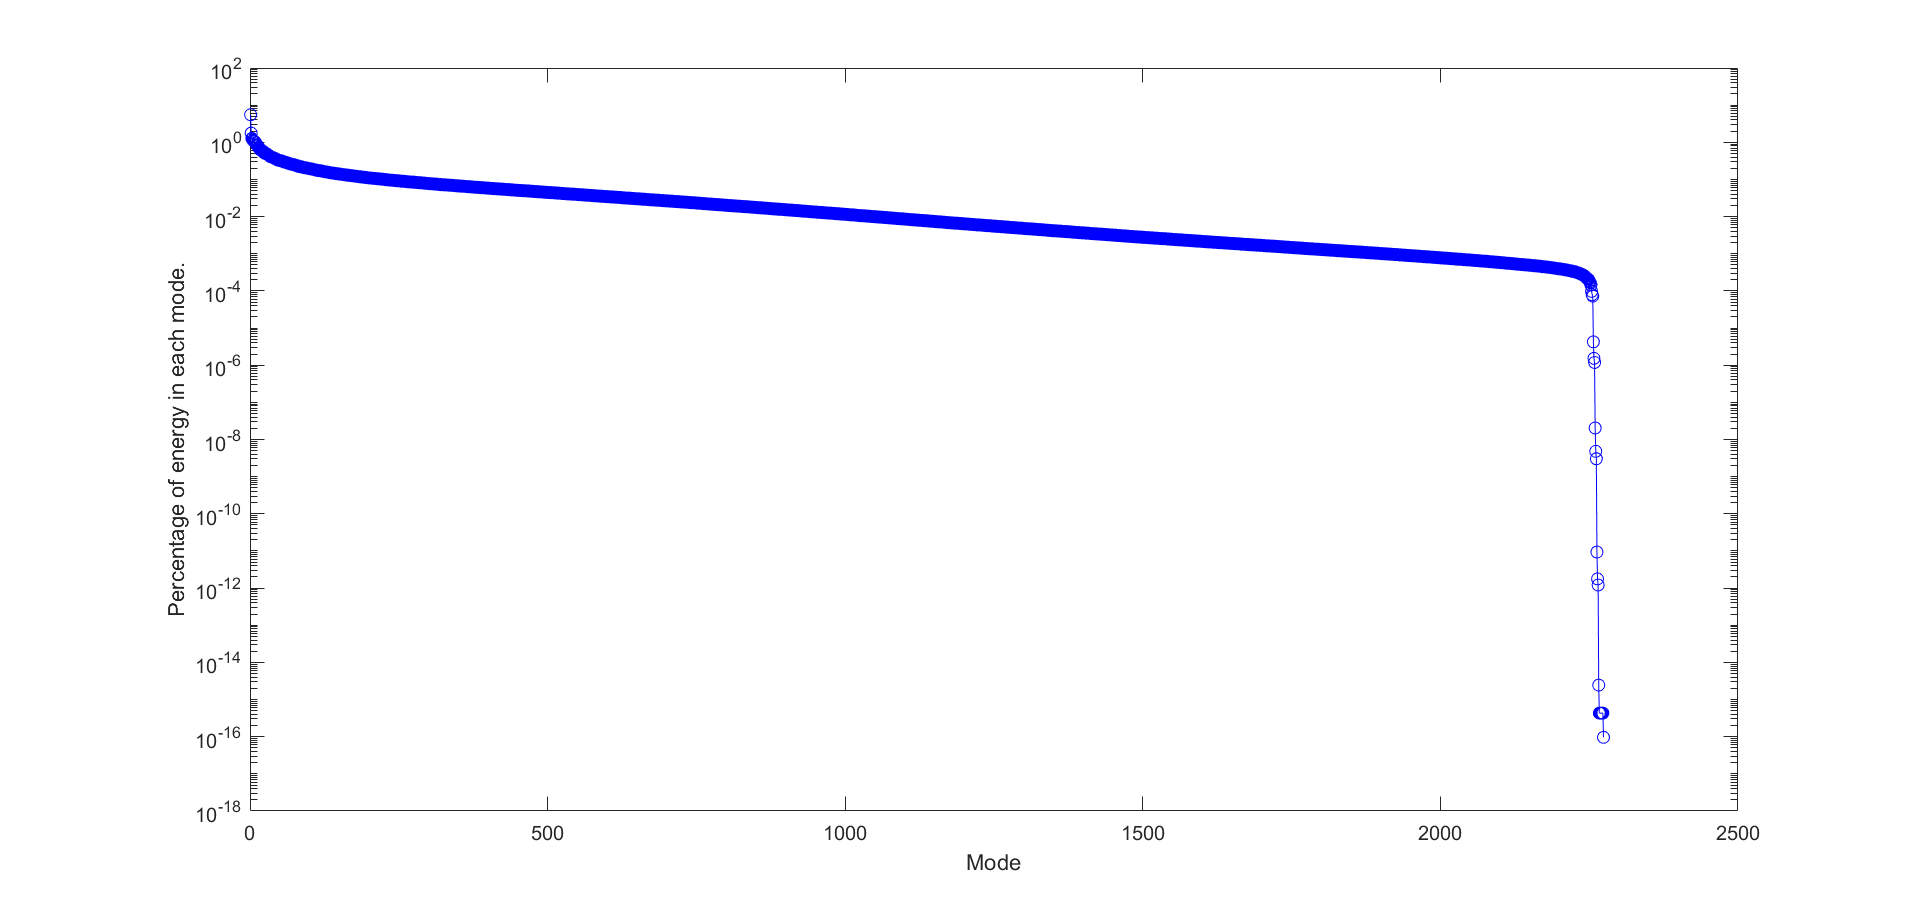
\includegraphics[width = 0.5\linewidth]{./Figures/test2_sigma.png}} 
\subfloat[First 3 principal components.]{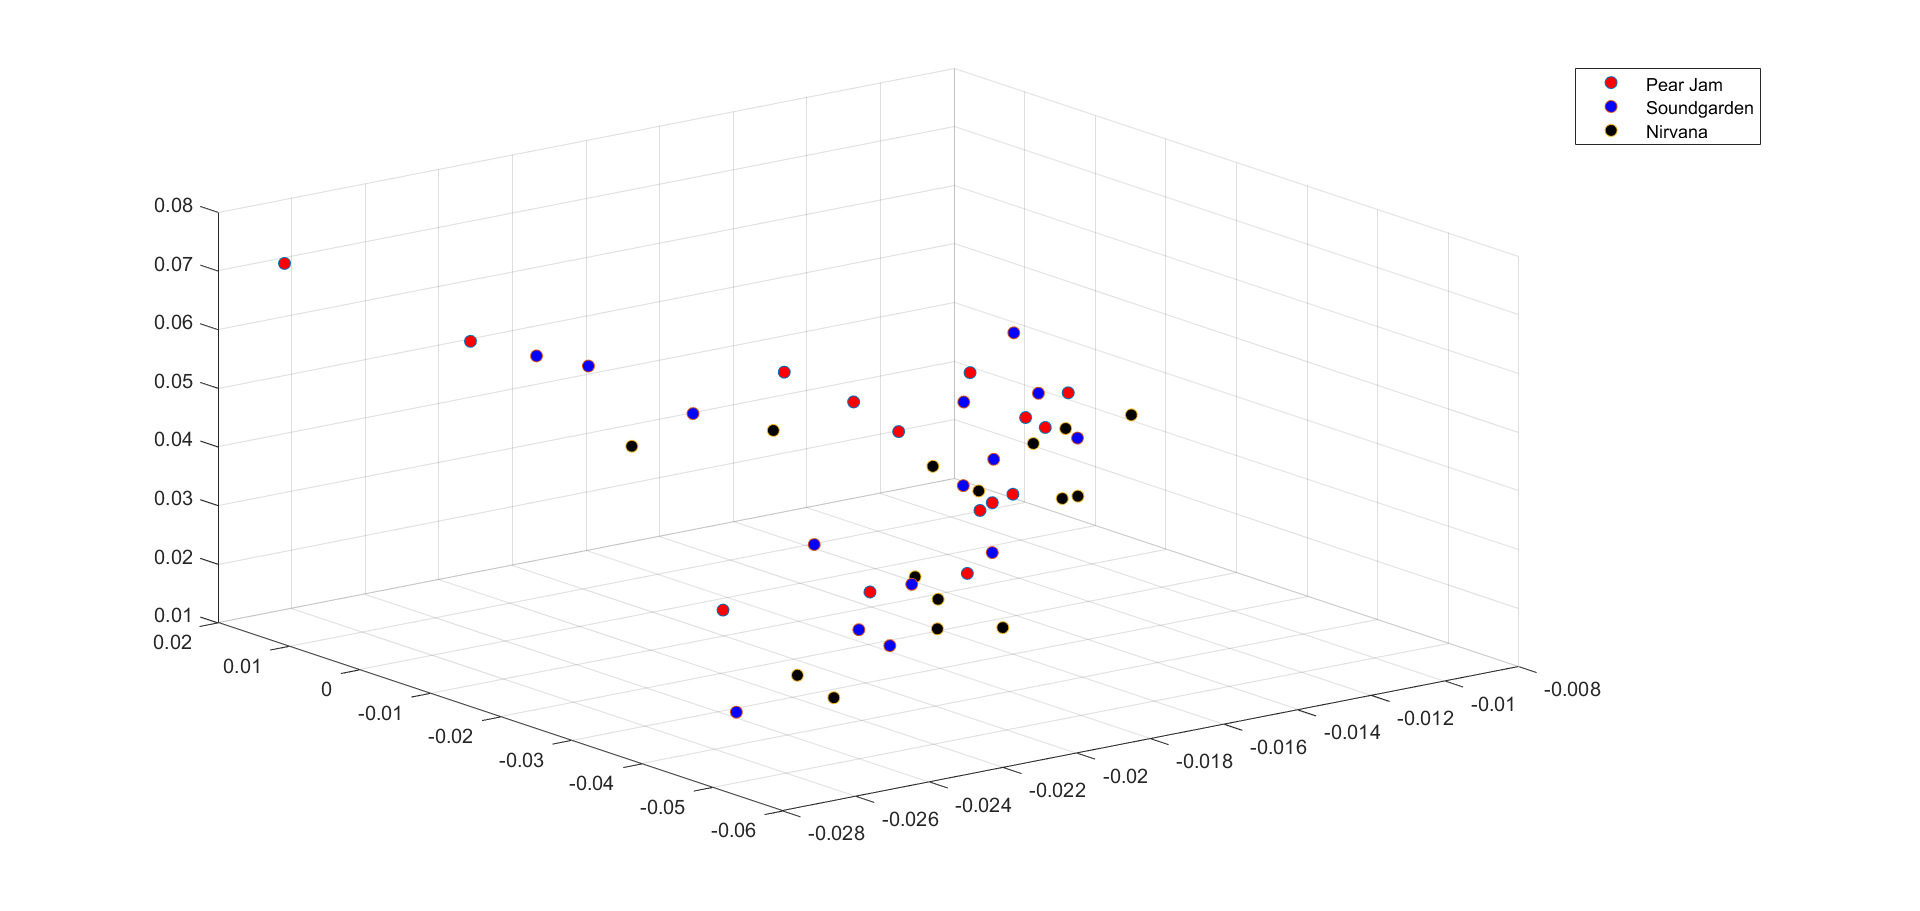
\includegraphics[width = 0.5\linewidth]{./Figures/test2_modes.png}}\\
\caption{Principal Component Analysis for Test 2. NB clasifier was trained with music from three bands of same genre.}
\label{fig:test2}
\end{figure}

\textbf{Test 3: Train NB classifier with music from multiple bands of different genres.}
Figure \ref{fig:test3}(a) shows the percentage of total energy contained in each modes. It was found that the classification error was smallest when $5$ principal components were used. The accurancy of NB classifier was found to be $\approx 68 \%$ with standard deviation of $\approx 15 \%$. Figure \ref{fig:test3}(b) shows how much the first $3$ principal components of the music of three bands from different genre are correlated. Figure \ref{fig:classification} compares the true classification with the predicted classification. \\
 
\begin{figure}[!b]
\subfloat[Percentage of variance captured by each mode.]{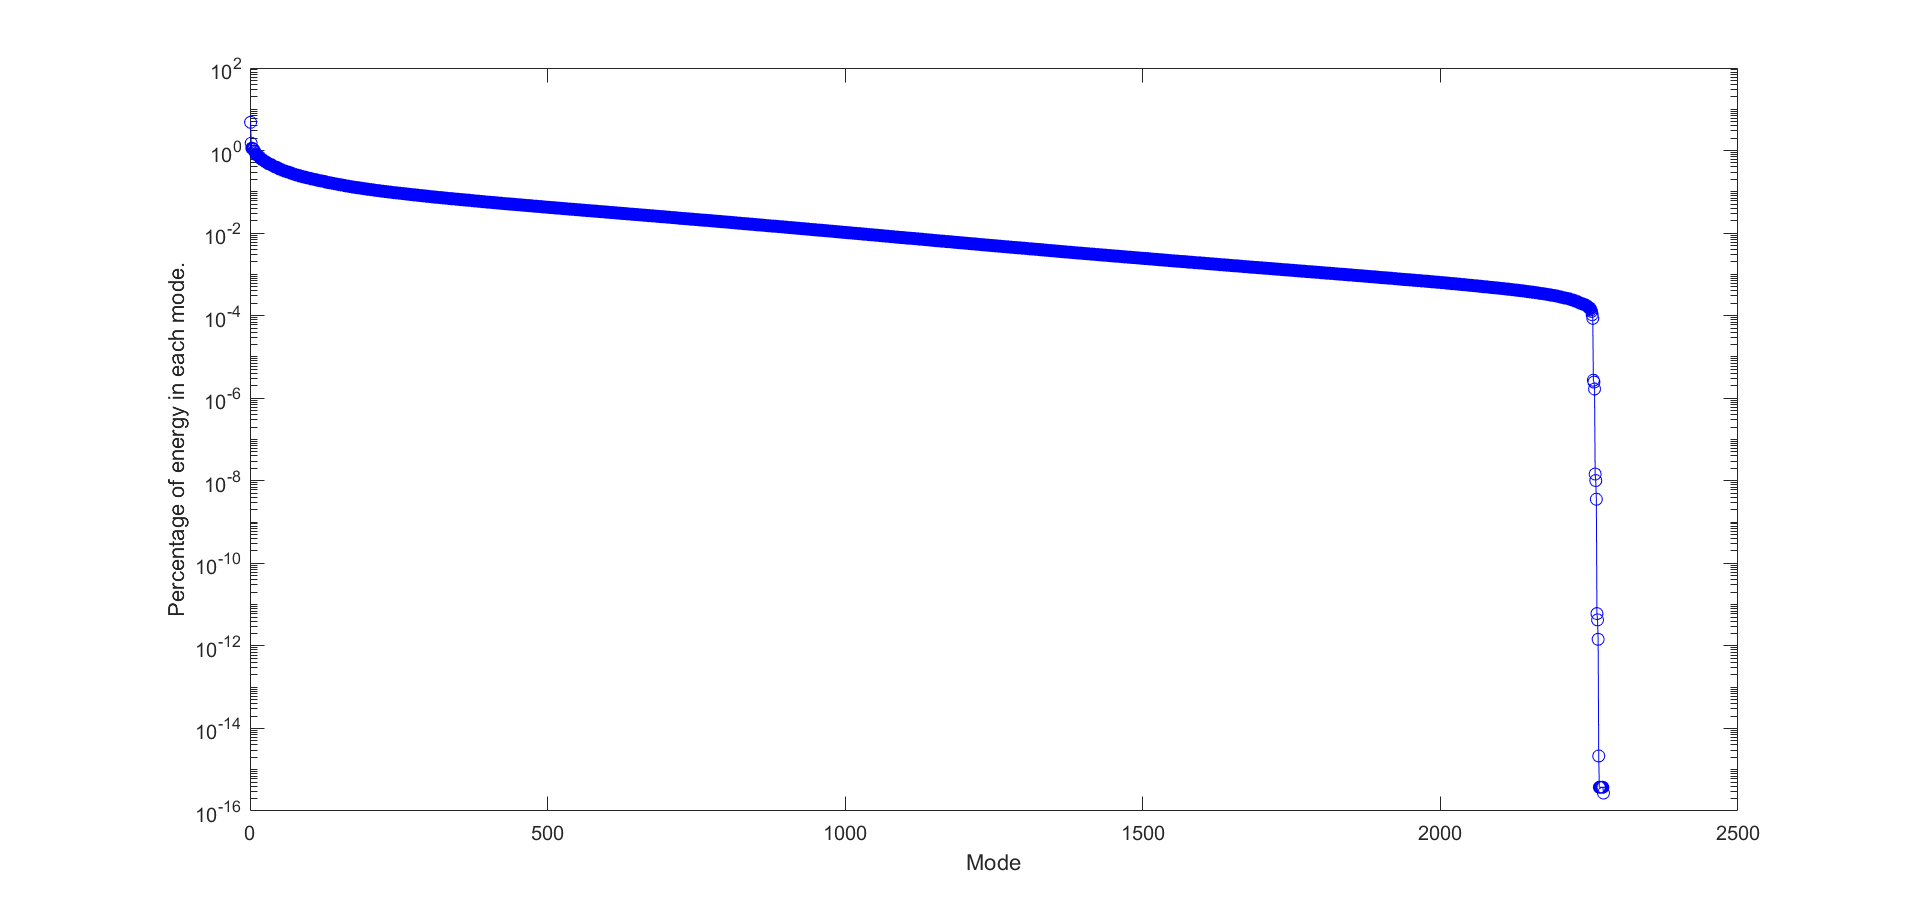
\includegraphics[width = 0.5\linewidth]{./Figures/test3_sigma.png}} 
\subfloat[First 3 principal components.]{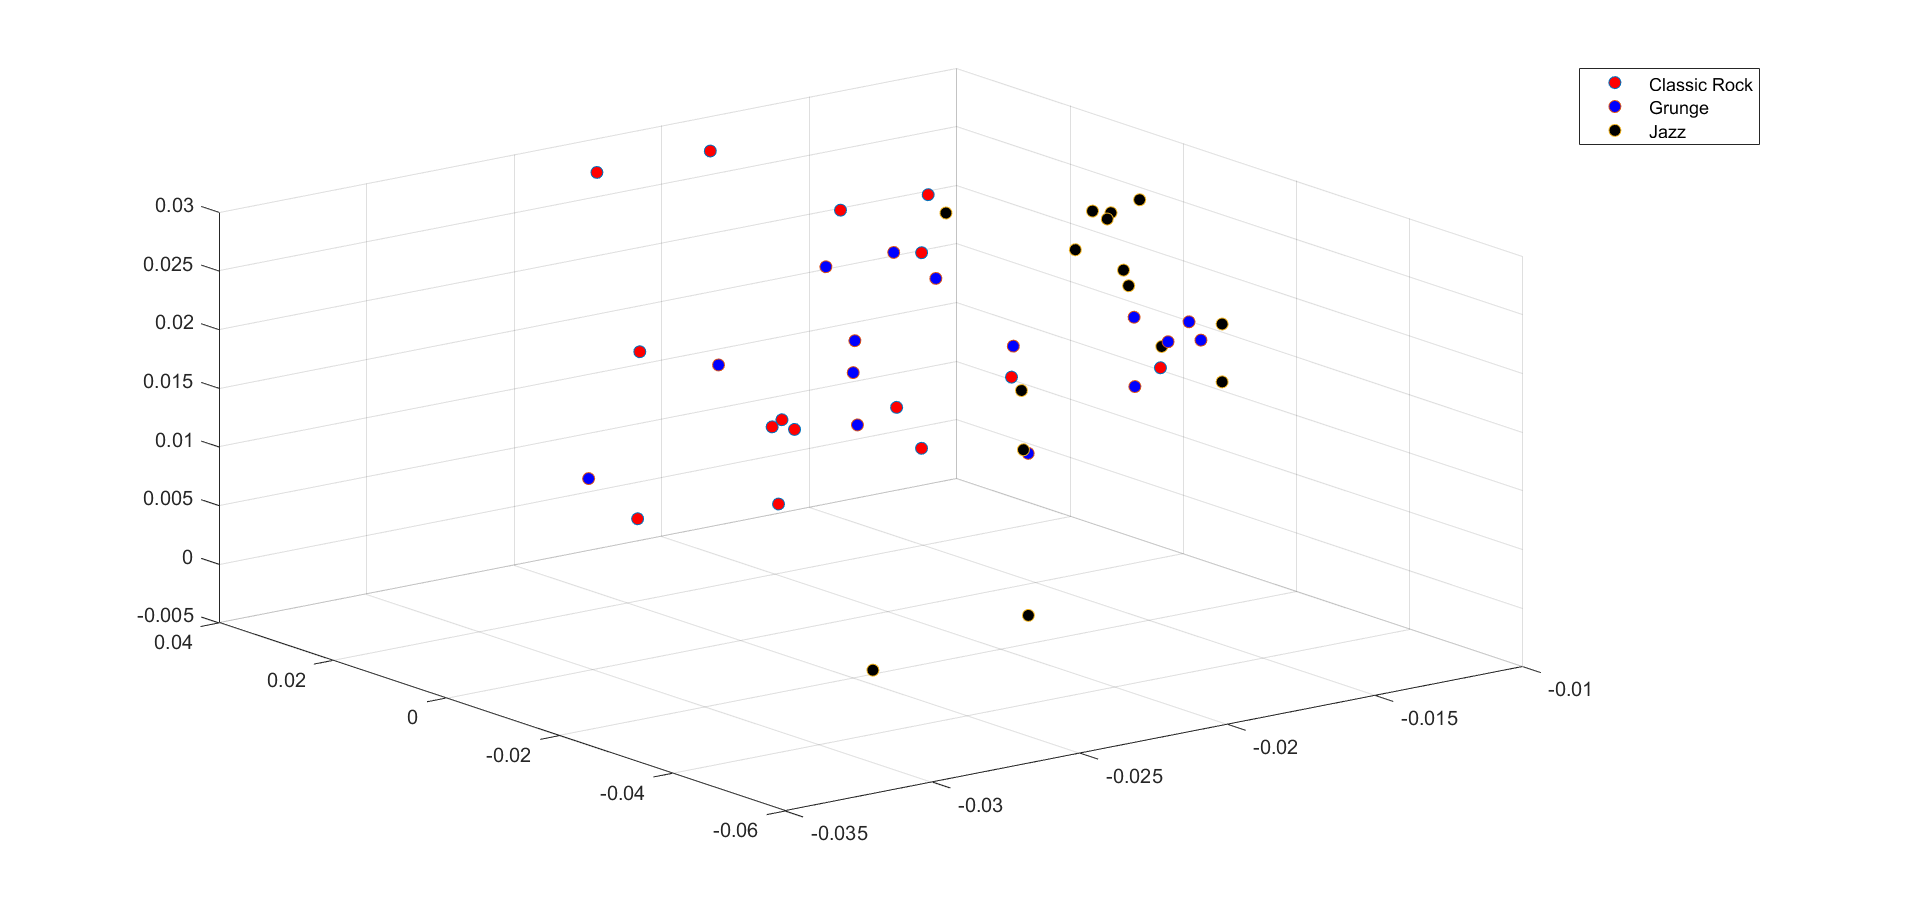
\includegraphics[width = 0.5\linewidth]{./Figures/test3_modes.png}}\\
\caption{Principal Component Analysis for Test 1. NB clasifier was trained with music from three bands of different genre.}
\label{fig:test3}
\end{figure}

\begin{figure}[!b]
\subfloat[True Classification.]{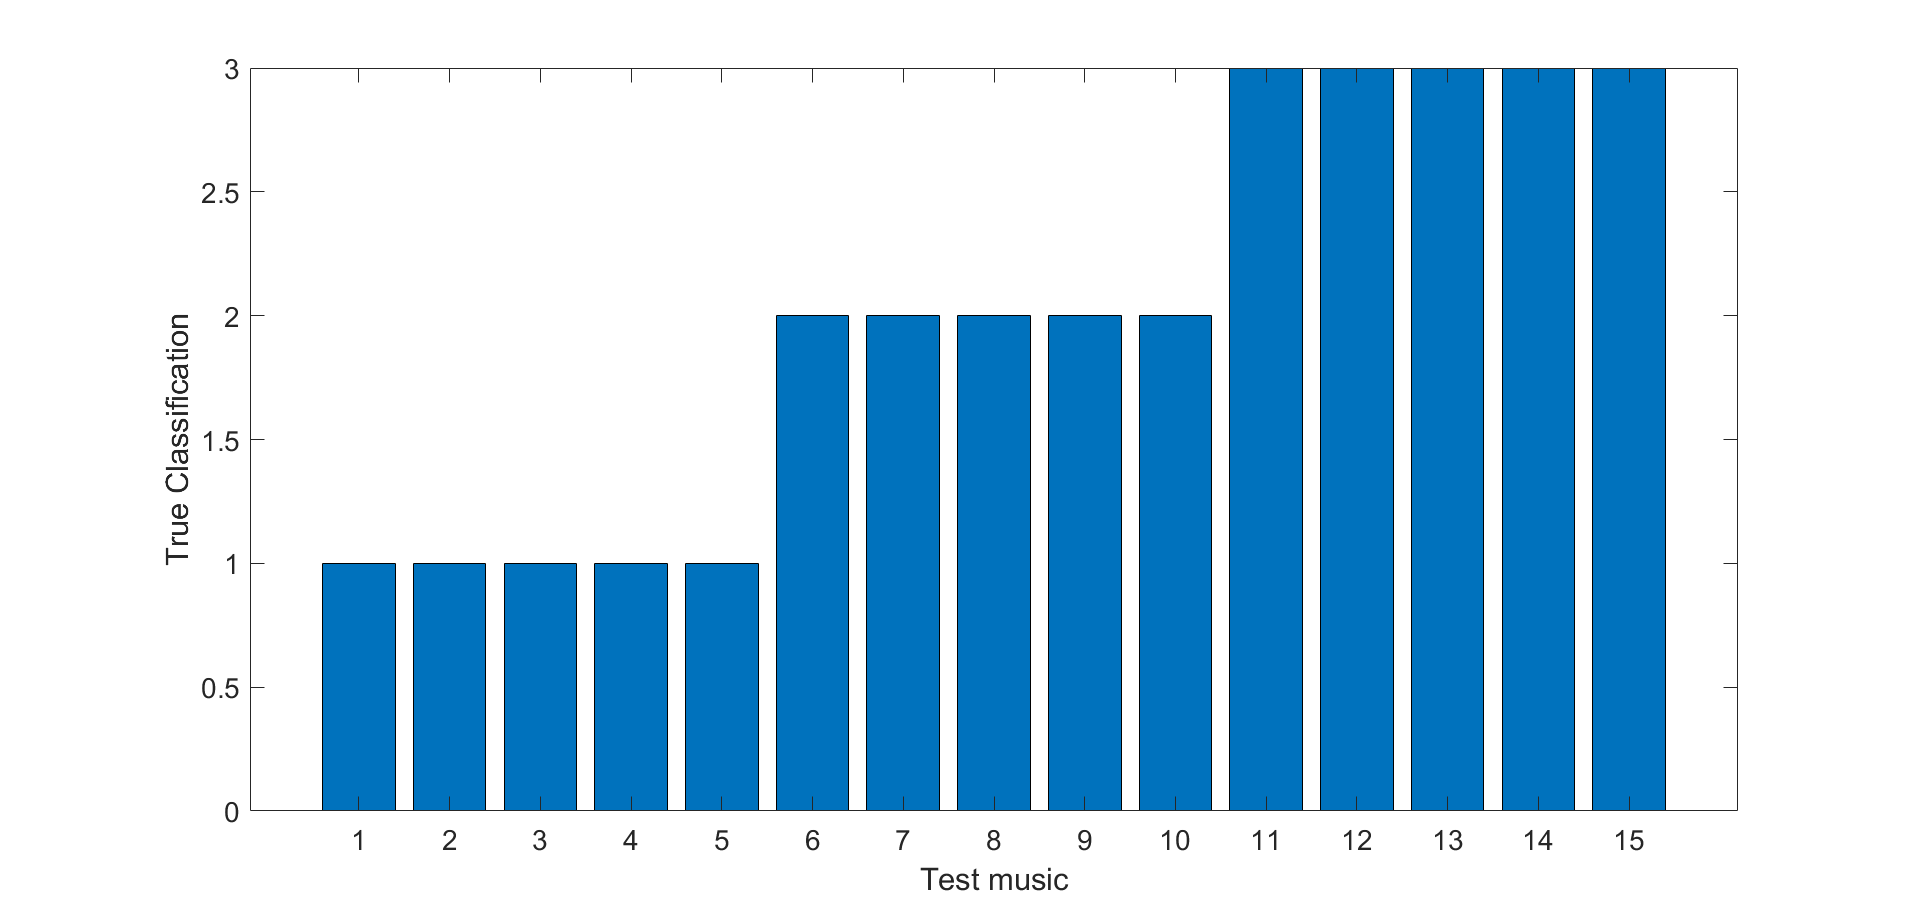
\includegraphics[width = 0.5\linewidth]{./Figures/test_truth.png}} 
\subfloat[Predicted Classification.]{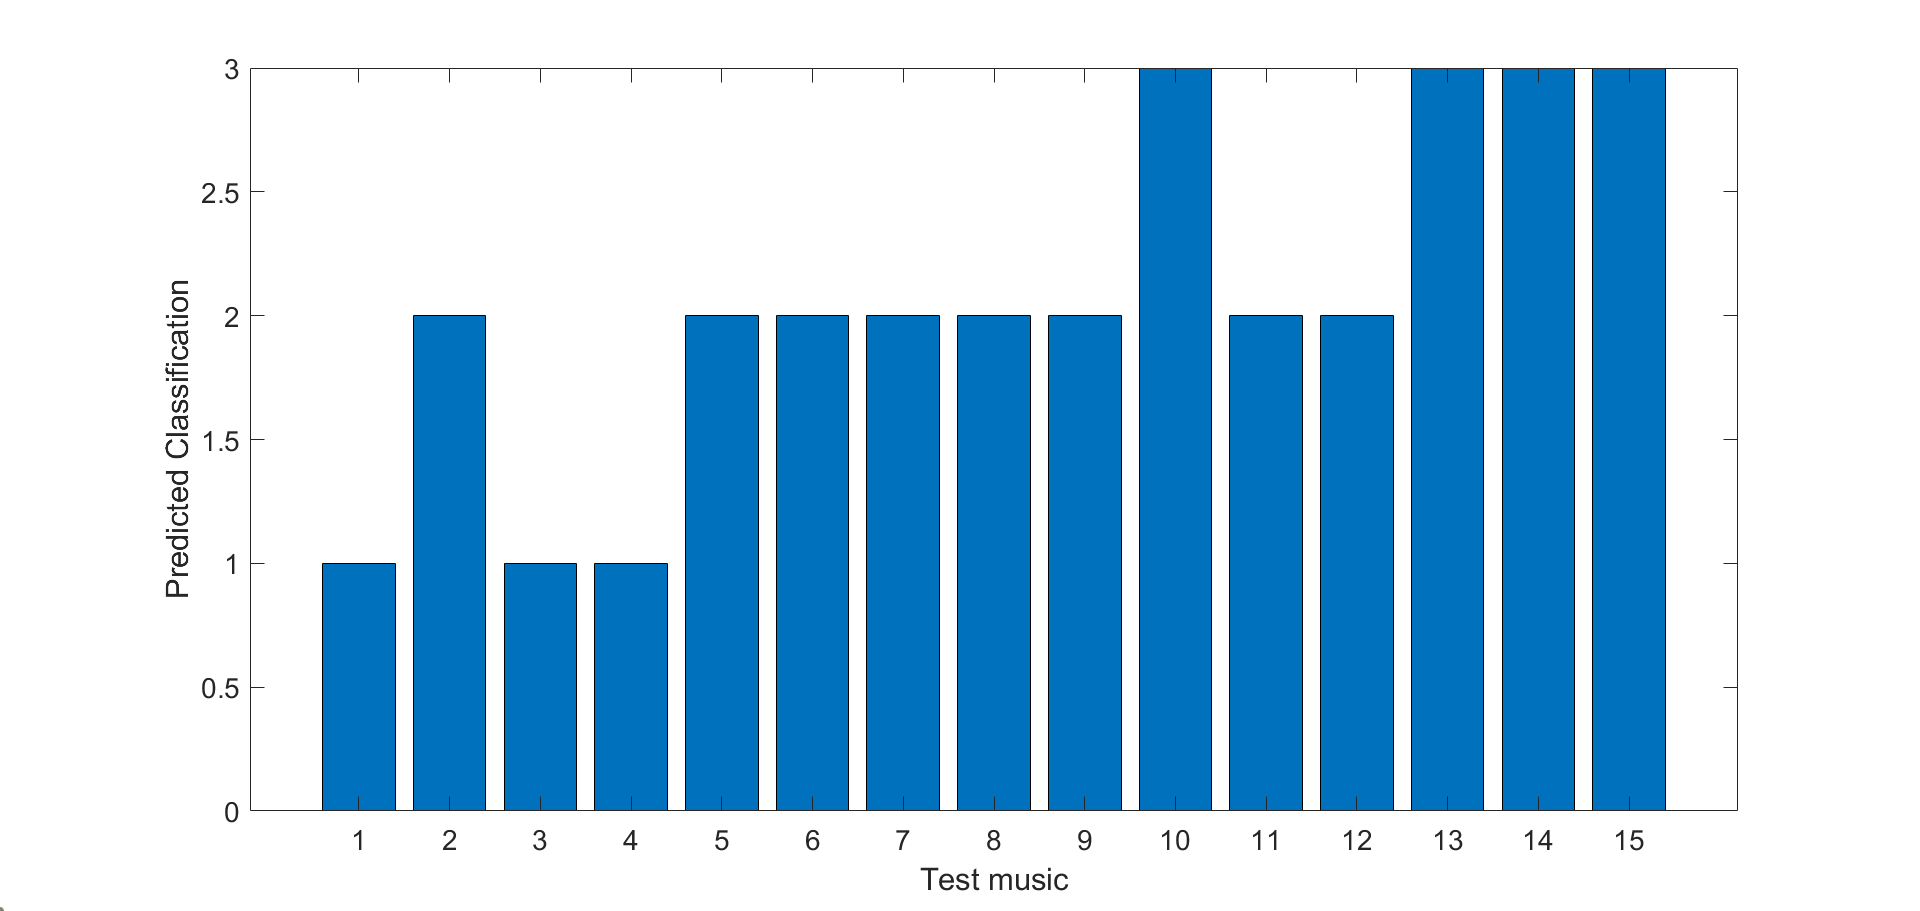
\includegraphics[width = 0.5\linewidth]{./Figures/test3_predict.png}}\\
\caption{Naive Bayes Classification for Test 3.}
\label{fig:classification}
\end{figure}


\pagebreak
% Summary and Conclusions
\section{Summary and Conclusions}
In this paper, Singular Value Decomposition (SVD) was analyzed as a learning algorithm. An image matrix, in which each column represents an image, was singularly decomposed to find the set of eigenfaces. These eigenfaces were then used to find low-dimensional approximation of a test image. Eigenfaces were generated for both cropped and un-cropped image datasets to study the effect of reflections, misalignment and background. SVD was also studied in the context of music genre classification. A Naive Bayes classification algorithm was implemented to classify a short piece of test music. The classifier was trained with three different datasets and its classification accuracy was compared. It was found that NB classifier was most acccurate when trained with music that was sampled from multiple bands across $3$ genres of music. More clustered the principal components, poorer the accuracy of the classification.

\begin{figure}[!b]
\subfloat[True Classification.]{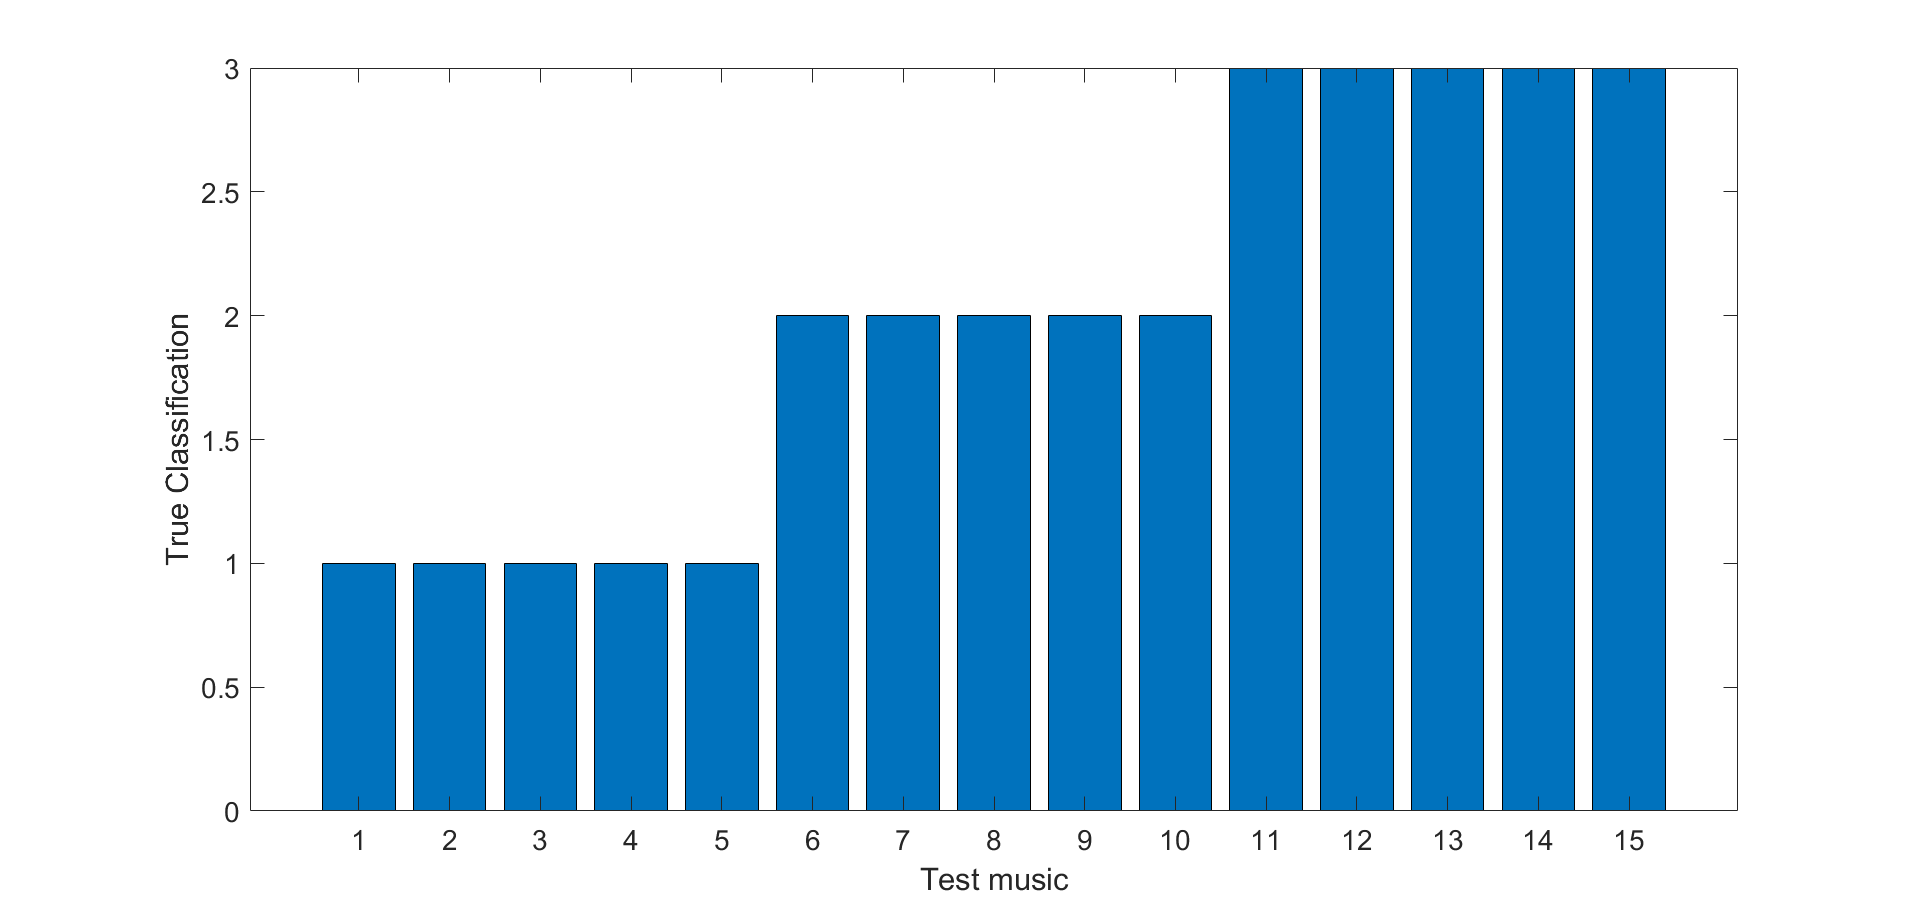
\includegraphics[width = 0.5\linewidth]{./Figures/test_truth.png}} 
\subfloat[Predicted Classification.]{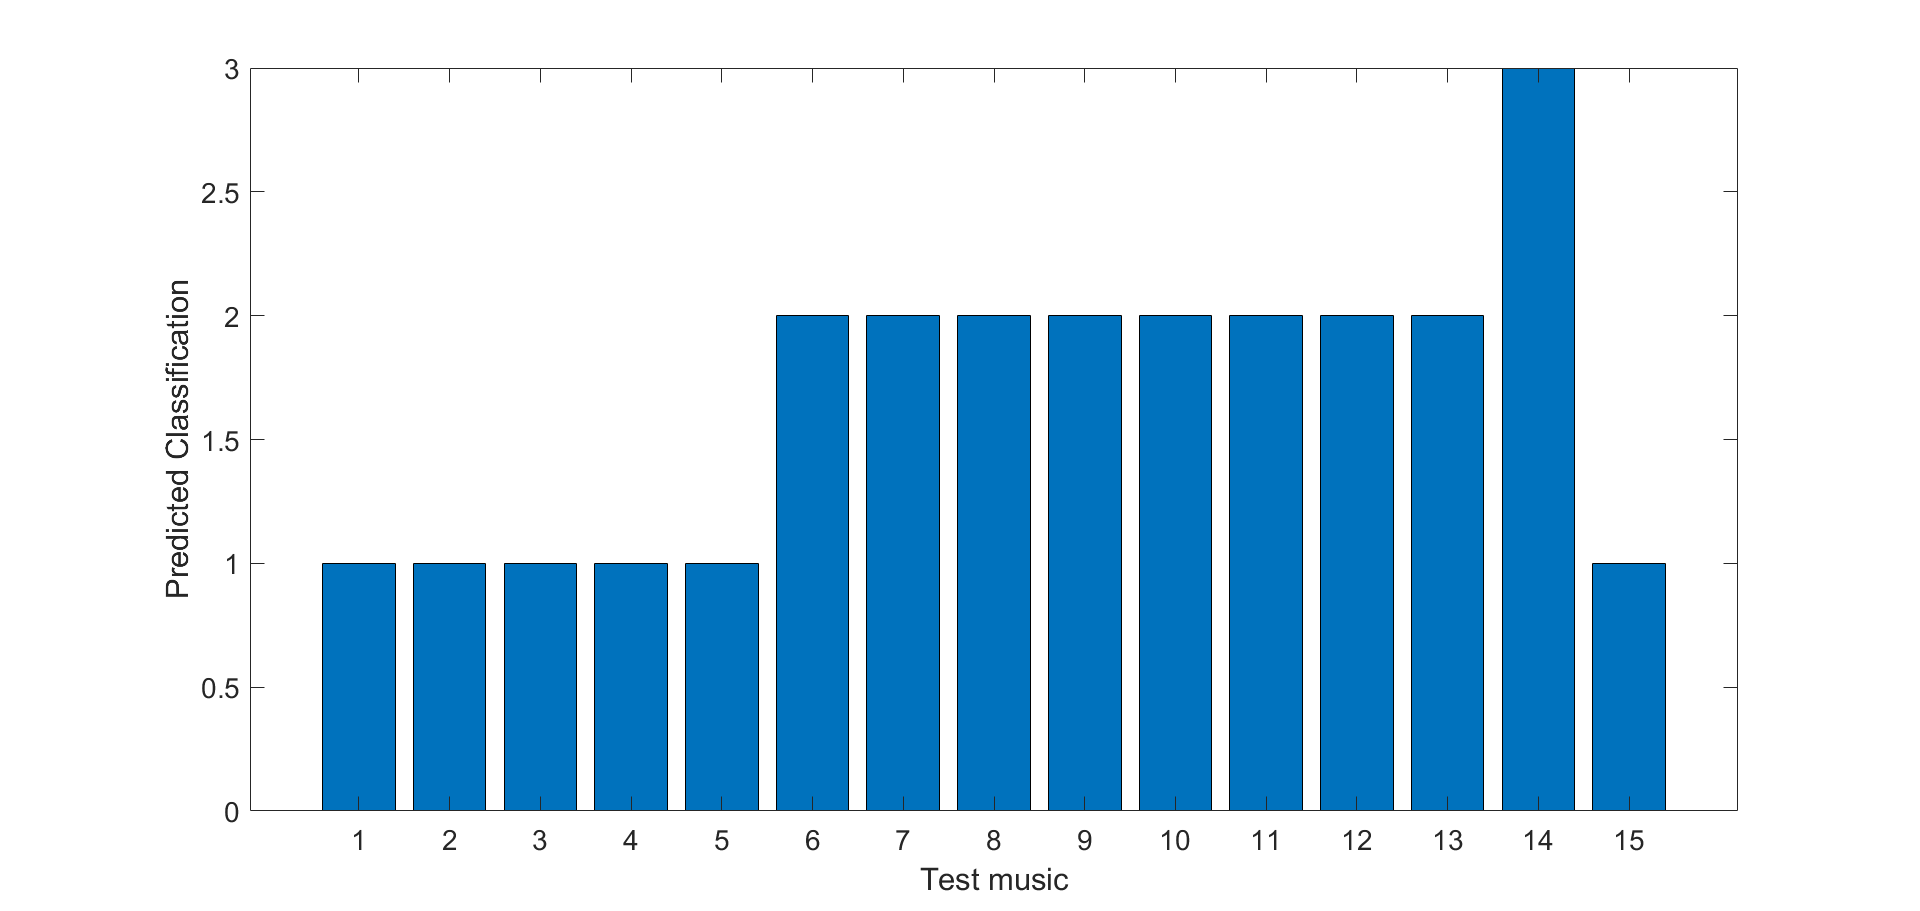
\includegraphics[width = 0.5\linewidth]{./Figures/test1_predict.png}}\\
\caption{Naive Bayes Classification for Test 1.}
\label{fig:classification1}
\end{figure}

\begin{figure}[!b]
\subfloat[True Classification.]{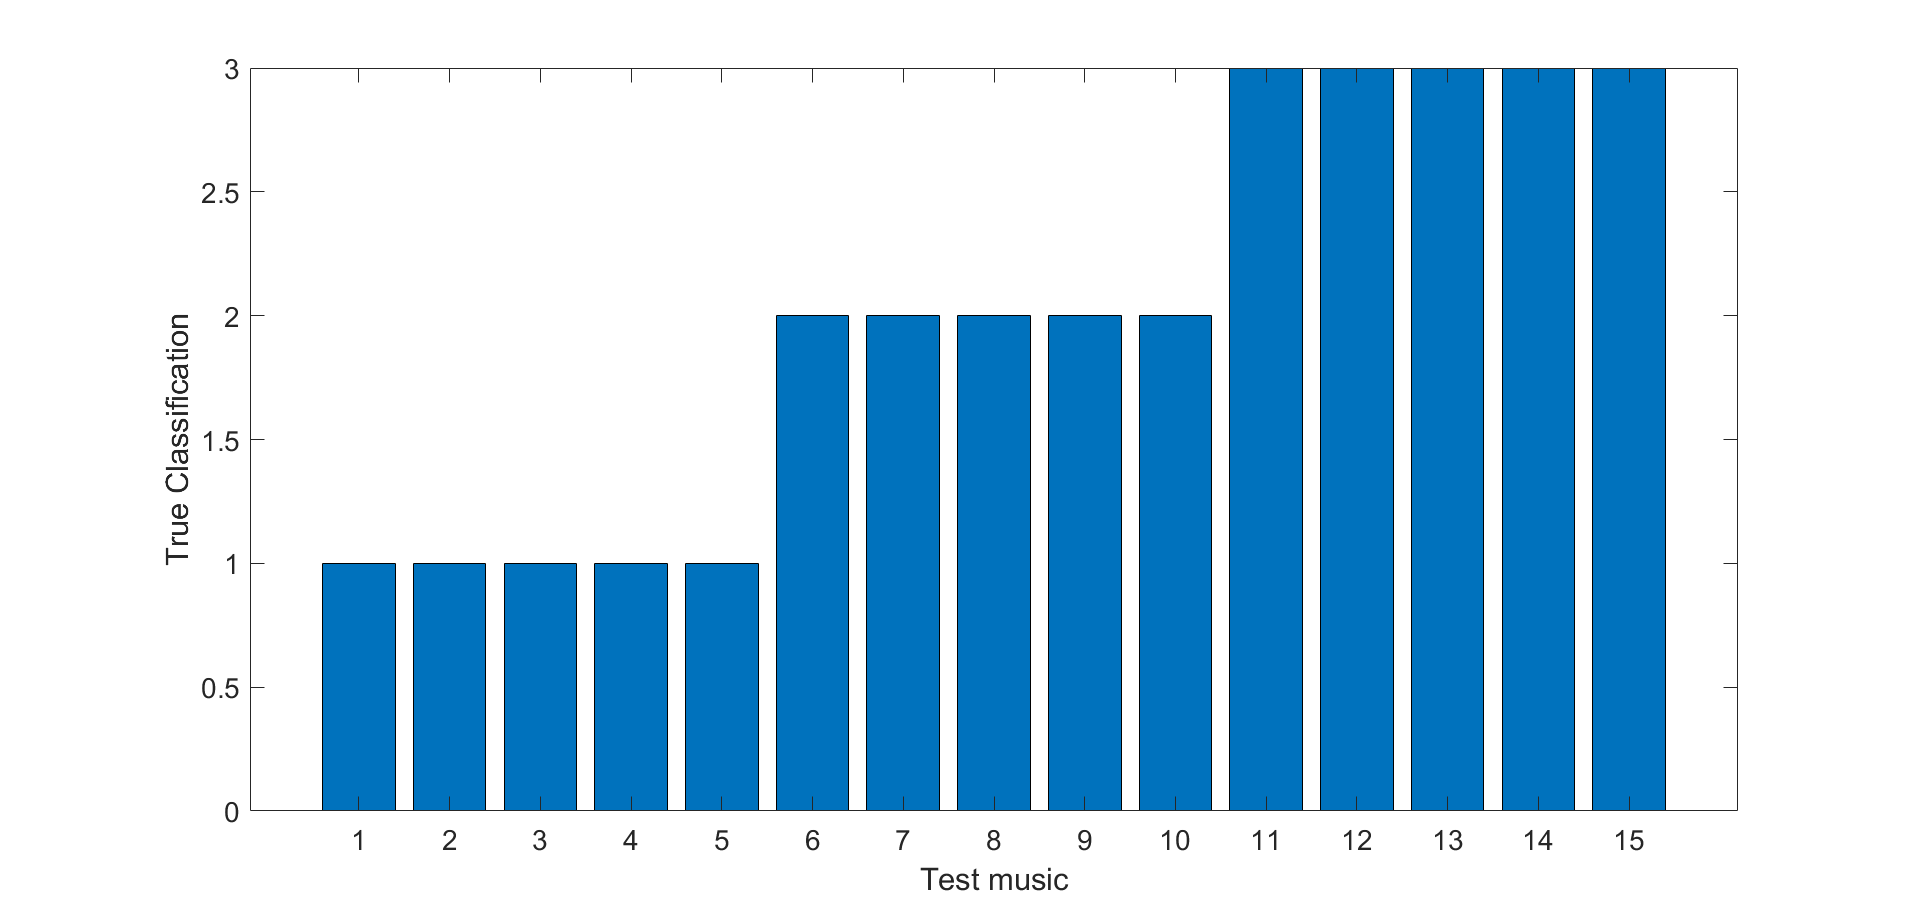
\includegraphics[width = 0.5\linewidth]{./Figures/test_truth.png}} 
\subfloat[Predicted Classification.]{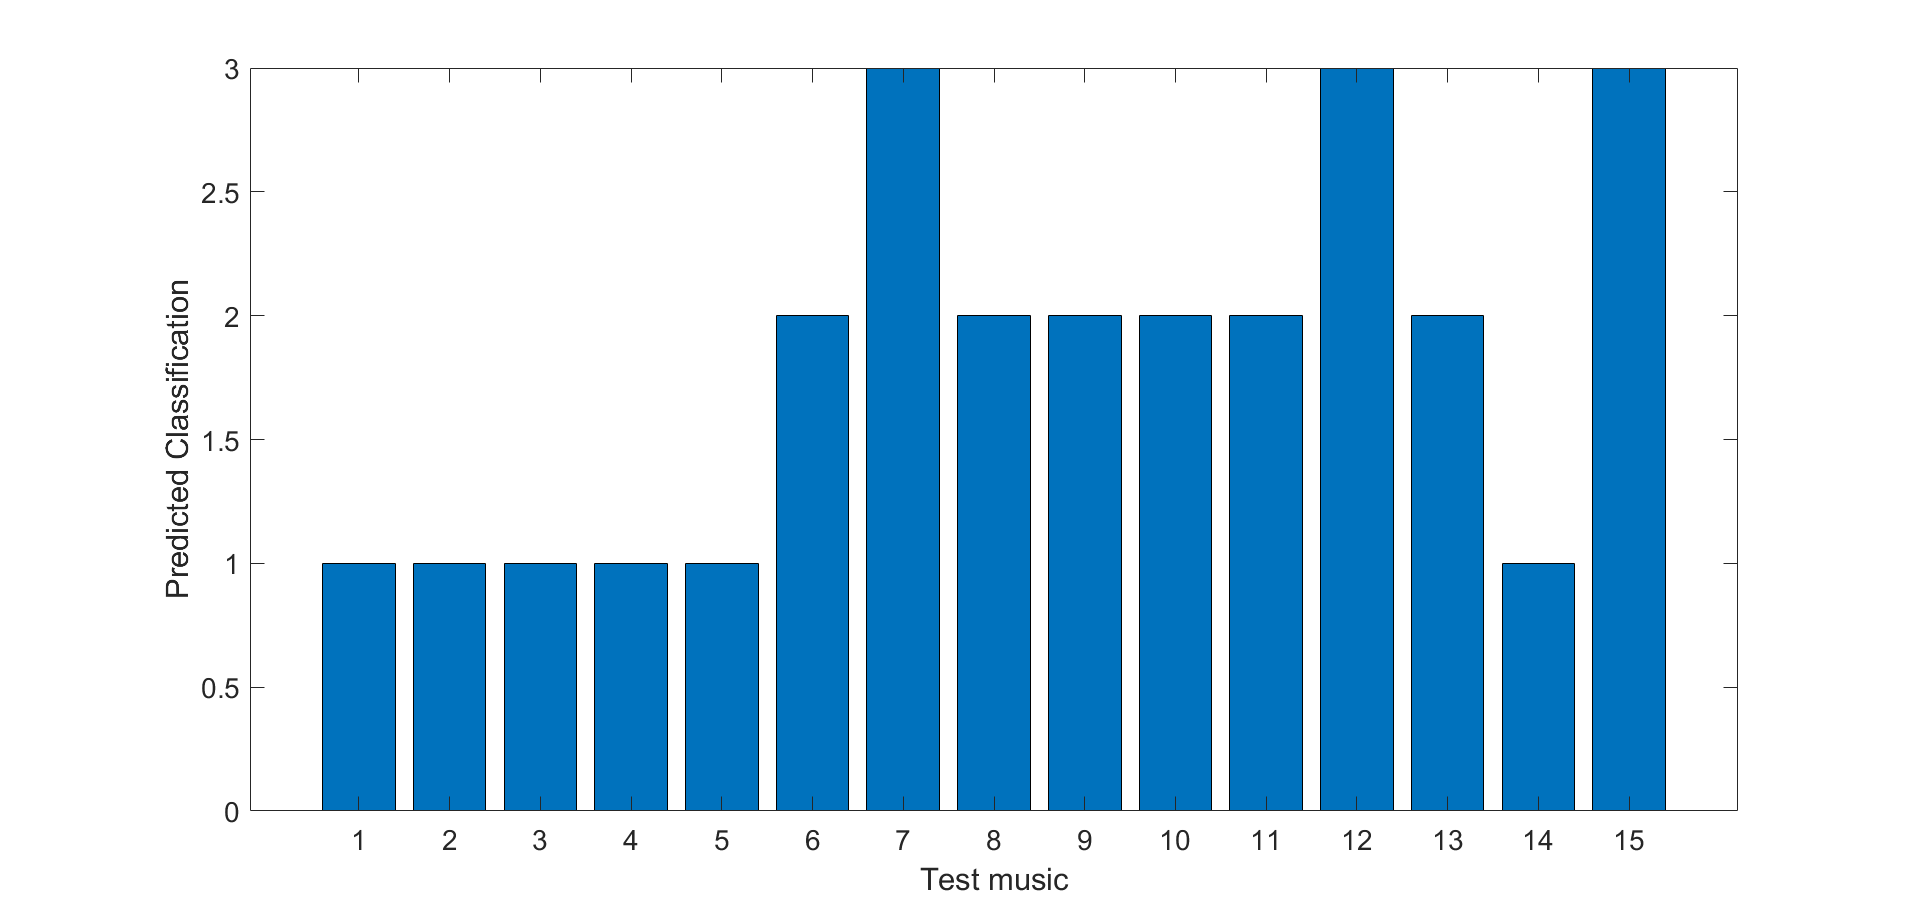
\includegraphics[width = 0.5\linewidth]{./Figures/test2_predict.png}}\\
\caption{Naive Bayes Classification for Test 2.}
\label{fig:classification2}
\end{figure} 

\pagebreak
% Appendices
\begin{appendices}

% MATLAB Functions
\section{MATLAB Functions}
Some important MATLAB functions used during the implementation.
\begin{itemize}
\item \texttt{y = linspace(x1,x2,n)} returns a row vector of \texttt{n} evenly spaced points between \texttt{x1} and \texttt{x2}. 
\item \texttt{ks = fftshift(k)} rearranges FT by shifting zero frequency component to the center of the array. Exchanges two halves of the array.
\item \texttt{Y = fftn(X)} returns multidimensional Fourier transform of an N-D array using FFT algorithm.
\item \texttt{[U,S,V] = svd(A)} performs a singular value decomposition of matrix A, such that A = U*S*V'.
\item \texttt{B = repmat(A,r1,...,rN)} specifies a list of scalars, r1,..,rN, that describes how copies of A are arranged in each dimension. When A has N dimensions, the size of B is size(A).*[r1...rN]. For example, repmat([1 2; 3 4],2,3) returns a 4-by-6 matrix.
\item \texttt{plot3(X,Y,Z)} plots coordinates in 3-D space.
\item \texttt{saveas(fig,filename,formattype)} creates the file using the specified file format, formattype
\item \texttt{dir} lists files and folders in the current folder.
\item \texttt{bar(y)} creates a bar graph with one bar for each element in y. If y is an m-by-n matrix, then bar creates m groups of n bars.
\item \texttt{imagesc(C)} displays the data in array C as an image that uses the full range of colors in the colormap
\end{itemize}

\pagebreak
% MATLAB Codes

\section{MATLAB Code}
\href{https://github.com/cssubedi/AMATH-582}{The code is published on the github repository AMATH-582 under Music Classification directory.} \\

\textbf{MATLAB code for Eigenfaces problem.}
\lstinputlisting[style=Matlab-editor]{yale_faces_cropped.m}
\lstinputlisting[style=Matlab-editor]{yale_faces_uncropped.m}
\pagebreak
\textbf{MATLAB code for Music Classification.}
\lstinputlisting[style=Matlab-editor]{music_classification.m}


\end{appendices}

\end{document}
